% GNN-AoI: complete project guide
% Compile: tectonic main.tex
\documentclass[11pt,a4paper]{article}
\usepackage[margin=2.2cm]{geometry}
\usepackage{amsmath,amssymb,bm}
\usepackage{graphicx}
\usepackage{float}
\usepackage{booktabs,longtable,tabularx,array,makecell}
\usepackage[dvipsnames]{xcolor}
\usepackage[most]{tcolorbox}
\usepackage{enumitem}
\usepackage{algorithm}
\usepackage{algpseudocode}
\usepackage{tikz}
\usetikzlibrary{arrows.meta,positioning,calc}
\usepackage{titlesec}
\usepackage{fancyhdr}
\usepackage[colorlinks=true,linkcolor=NavyBlue,urlcolor=NavyBlue,citecolor=NavyBlue]{hyperref}

\graphicspath{{../results/figures/}{../presentation/figures/}}
\setlength{\parskip}{0.45em}
\setlength{\parindent}{0pt}
\setlist{itemsep=0.2em,topsep=0.3em}
\renewcommand{\arraystretch}{1.18}

\definecolor{accent}{HTML}{2563EB}
\titleformat{\section}{\Large\bfseries\color{accent}}{\thesection}{0.6em}{}
\titleformat{\subsection}{\large\bfseries}{\thesubsection}{0.6em}{}
\titleformat{\subsubsection}{\normalsize\bfseries}{\thesubsubsection}{0.6em}{}

\pagestyle{fancy}
\fancyhf{}
\fancyhead[L]{}
\fancyhead[R]{\small\color{gray}GNN-AoI: Complete Project Guide \ $\cdot$\ \nouppercase{\leftmark}}
\fancyfoot[C]{\small\thepage}
\renewcommand{\headrulewidth}{0.3pt}

\newtcolorbox{whybox}[1][Why?]{colback=blue!4,colframe=blue!55!black,fonttitle=\bfseries,title={#1},breakable,
  left=6pt,right=6pt,top=4pt,bottom=4pt}
\newtcolorbox{saybox}[1][How to explain it to your faculty]{colback=green!5,colframe=green!45!black,fonttitle=\bfseries,
  title={#1},breakable,left=6pt,right=6pt,top=4pt,bottom=4pt}
\newtcolorbox{notebox}[1][Note]{colback=orange!6,colframe=orange!70!black,fonttitle=\bfseries,title={#1},breakable,
  left=6pt,right=6pt,top=4pt,bottom=4pt}
\newtcolorbox{keybox}[1][Key idea]{colback=gray!6,colframe=gray!60!black,fonttitle=\bfseries,title={#1},breakable,
  left=6pt,right=6pt,top=4pt,bottom=4pt}

\newcommand{\fig}[3][\textwidth]{\begin{figure}[htbp]\centering\includegraphics[width=#1]{#2}\caption{#3}\end{figure}}
\renewcommand{\cite}[1]{[#1]}
\newcommand{\Acorr}{A_{\mathrm{corr}}}
\newcommand{\Apost}{A_{\mathrm{post}}}

\begin{document}

\begin{titlepage}
  \centering
  \vspace*{2cm}
  {\color{accent}\large\bfseries COMPLETE PROJECT GUIDE\par}
  \vspace{0.8cm}
  {\Huge\bfseries GNN-AoI\par}
  \vspace{0.4cm}
  {\LARGE Correlation-Aware Scheduling of\\ Real Sensor Networks\par}
  \vspace{0.6cm}
  {\large A graph neural network, trained with reinforcement learning, that decides which sensors may
  transmit, while every sensor stays fresh by construction\par}
  \vspace{1.5cm}
  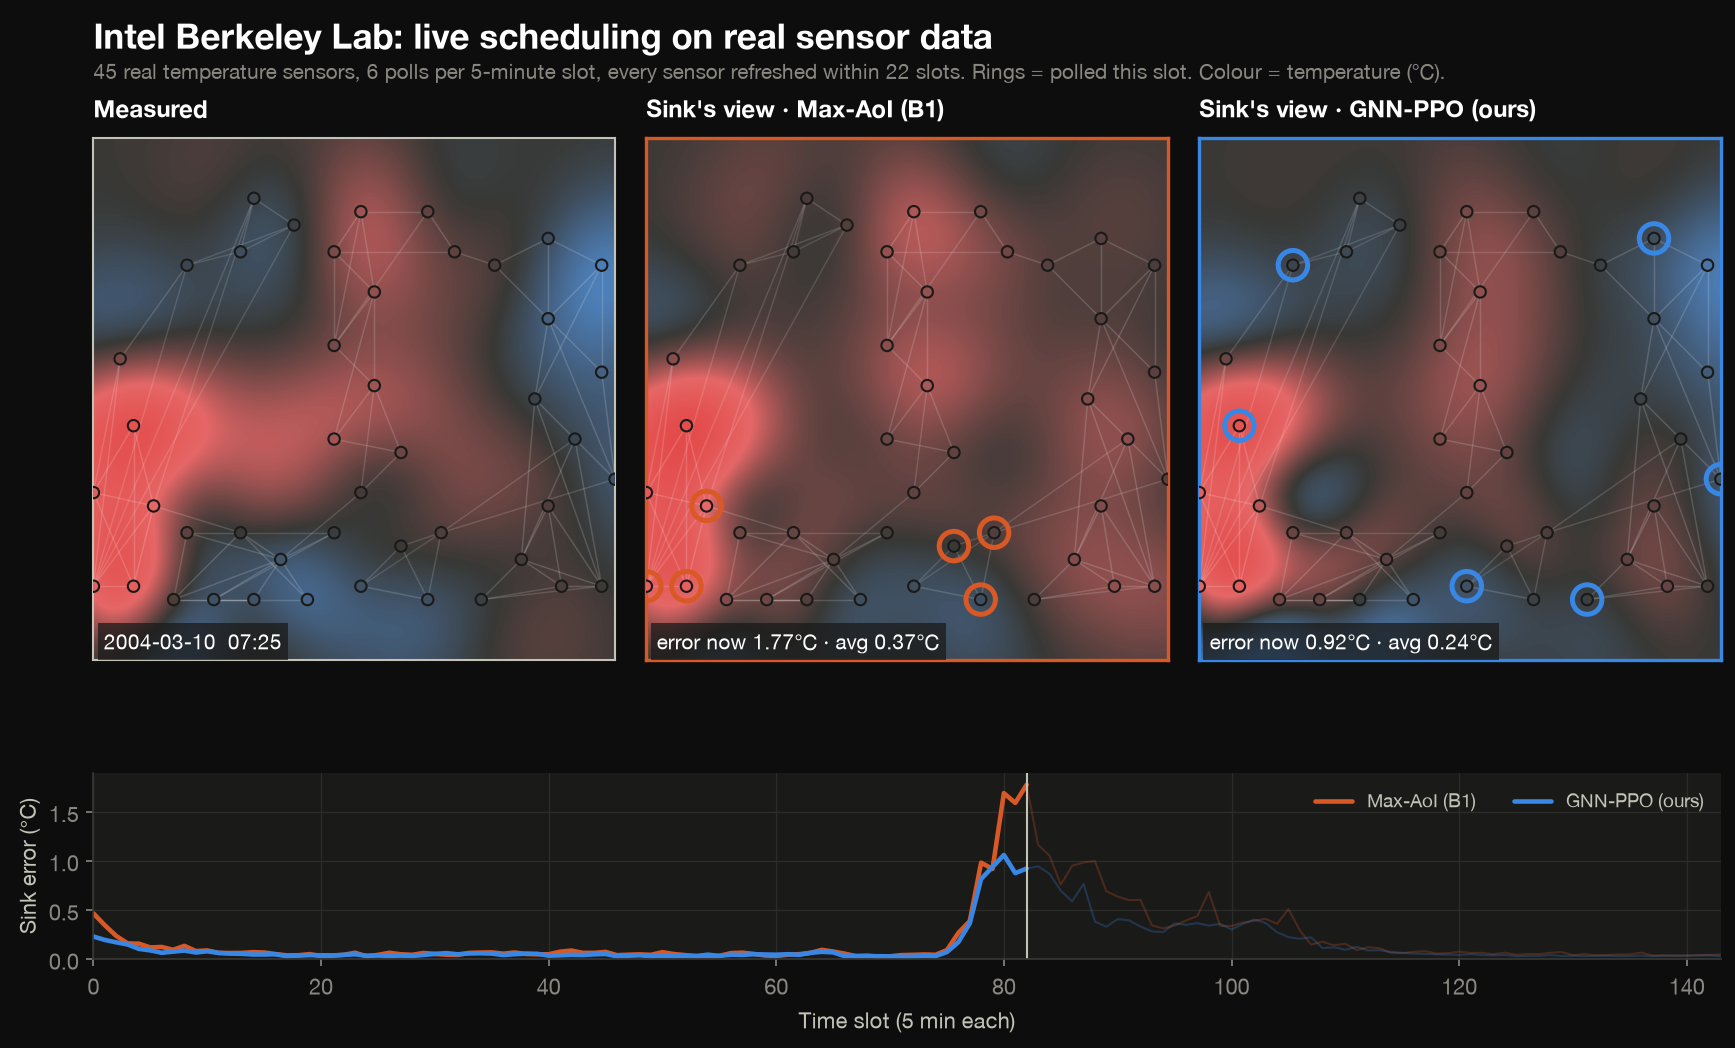
\includegraphics[width=0.85\textwidth]{hero.png}
  \vspace{1.5cm}

  {\large\bfseries Bhanu Prasad Palella \quad Gullanki Bhagya Lakshmi\\[0.3em] Pavna Preethikha \quad Madhumitha S\par}
  \vspace{0.5cm}
  {\large Amrita School of Artificial Intelligence\par}
  \vspace{0.3cm}
  {\normalsize Guide: [guide's name]\par}
  \vfill
  {\small Everything about the project: the problem, the research gaps, the objectives, the full methodology,
  every implementation step and design decision, every result and how to explain it.\par}
\end{titlepage}

\tableofcontents
\newpage

\section{Introduction}
\subsection{How to read this guide}

This guide explains the whole GNN-AoI project from zero. Read it in order the first time; afterwards use the
contents page to jump to what you need.

\begin{itemize}
  \item \textbf{Section 2} is the glossary: every abbreviation and technical term used anywhere in the project.
  \item \textbf{Section 3} teaches the background ideas (sensor networks, Age of Information, correlation, Kalman
        filters, graph neural networks, reinforcement learning, PPO) from first principles.
  \item \textbf{Section 4} shows how the problem statement came out of the gaps in published research, and lists the
        objectives with how each one was achieved.
  \item \textbf{Section 5} is the complete methodology, equation by equation.
  \item \textbf{Section 6} is the implementation story, step by step, in the order we actually built it.
  \item \textbf{Section 7} explains every design decision: why this dataset, tool or algorithm, and why not the
        alternatives.
  \item \textbf{Section 8} covers the expected output, the obtained output, and every graph and table, with a
        ready-to-use explanation for your faculty.
  \item \textbf{Section 9} gives the conclusion, limitations, future work, likely viva questions and references.
\end{itemize}

Throughout the guide, three kinds of boxes appear:

\begin{whybox}[Why? boxes]
explain the reason behind a choice.
\end{whybox}
\begin{saybox}[How to explain it to your faculty]
give you sentences you can say almost word for word.
\end{saybox}
\begin{notebox}[Note boxes]
point out a subtle detail or an honest limitation.
\end{notebox}

\subsection{The project in one page}

\begin{keybox}[The problem in two sentences]
A base station (the \emph{sink}) must keep track of the readings of many sensors, but the wireless channel lets
only a few of them transmit in each time slot. Which sensors should transmit so that the sink knows the
\emph{whole} field as accurately as possible, while no sensor is ignored for too long?
\end{keybox}

\textbf{The usual answer and why it is not enough.} The standard approach is to poll whichever sensor has gone
longest without reporting. That keeps the \emph{Age of Information} (AoI) low, but it treats every sensor as
independent. In real networks, neighbouring sensors measure almost the same thing (two thermometers in the same room,
two traffic detectors on the same freeway). Polling both wastes a transmission: once one of them reports, the sink
can already infer the other quite well.

\textbf{Our answer.} GNN-AoI is a scheduler that:
\begin{enumerate}
  \item \textbf{learns from historical data} which sensors are correlated (a \emph{correlation graph});
  \item keeps a \textbf{Kalman filter} at the sink, which turns every received reading into an updated estimate of
        \emph{all} sensors, together with how uncertain it is about each one;
  \item uses a \textbf{graph neural network} (GNN) that looks at the graph and the sink's uncertainty and chooses
        which sensors transmit in each slot;
  \item trains that GNN with \textbf{reinforcement learning} (the PPO algorithm), rewarding it for low estimation
        error at the sink;
  \item enforces a \textbf{hard freshness guarantee}: every sensor must report at least once every $F$ slots, no
        matter what the scheduler would prefer.
\end{enumerate}

\textbf{Where we tested it.} On two real sensor datasets, using only time periods that were never used for
training: 45 temperature sensors in the Intel Berkeley Research Lab (2004), and 325 freeway speed sensors in the
San Francisco Bay Area (PEMS-BAY, 2017). We also tested on thousands of simulated sensor layouts.

\textbf{Headline results.}
\begin{center}
\small
\begin{tabular}{@{}lccc@{}}
  \toprule
  & \makecell{\textbf{Intel Lab}\\(45 sensors, $C=6$)} & \makecell{\textbf{PEMS-BAY}\\(325 sensors, $C=40$)} & \makecell{\textbf{Synthetic}\\($M=50$, $C=10$)} \\
  \midrule
  Max-AoI (classic) & 0.292\,$^\circ$C & 2.85 mph & 0.0399 (MSE) \\
  Kalman-greedy & 0.277\,$^\circ$C & 2.95 mph & 0.0205 \\
  \textbf{GNN-PPO (ours)} & \textbf{0.235\,$^\circ$C} & \textbf{2.78 mph} & \textbf{0.0200} \\
  Change vs.\ Max-AoI & $-20\%$ & $-2.4\%$ & $-50\%$ \\
  GNN beats Kalman-greedy in & 10/10 test windows & 15/15 test windows & 73\% of layouts \\
  \bottomrule
\end{tabular}
\end{center}
(Real-data numbers are the sink's root-mean-square error in physical units; lower is better.)

\textbf{What we built.} A tested, open-source Python package (\texttt{gnn\_aoi}) with the simulator, real-data
loaders, Kalman sink, five baseline schedulers, the GNN, the PPO trainer, all experiments and figures, and a live
web demo that replays a real day and shows every transmission as it happens.

\begin{saybox}
``Classic schedulers only ask \emph{who has been silent the longest}. We ask \emph{who would teach the sink the most
right now}, using correlations learned from real data, and we still guarantee that nobody stays silent too long.
On the real Intel lab data this lowers the sink's temperature error by 20 percent with the same channel and the same
freshness guarantee.''
\end{saybox}

\section{Abbreviations and important terms}

\subsection{Abbreviations}

{\small
\begin{longtable}{@{}p{2.6cm}p{5.2cm}p{7.6cm}@{}}
\toprule
\textbf{Short form} & \textbf{Full form} & \textbf{Meaning in this project} \\
\midrule
\endhead
AoI & Age of Information & Time (in slots) since the sink last received a reading from a sensor. \\
AoCI & Age of Correlated Information & A sensor is only as stale as its freshest correlated neighbour; an early, graph-based version of our idea (kept as a metric). \\
AoII & Age of Incorrect Information & Variant of AoI that only counts time during which the sink's knowledge is wrong \cite{17}. \\
PAoI & Peak Age of Information & The largest age reached before an update arrives. \\
WSN & Wireless Sensor Network & Many small sensors reporting over radio to a base station. \\
IoT & Internet of Things & Networked everyday devices and sensors. \\
CPS & Cyber-Physical System & A system where computation monitors or controls a physical process. \\
GNN & Graph Neural Network & A neural network that works on graphs by passing messages between connected nodes. \\
GCN & Graph Convolutional Network & A common GNN type \cite{21}. \\
MPNN & Message-Passing Neural Network & General GNN framework; ours is one. \\
MLP & Multi-Layer Perceptron & A plain feed-forward neural network. \\
GELU & Gaussian Error Linear Unit & The activation function used in our MLPs. \\
LN & Layer Normalisation & Rescales each node's embedding to stabilise training. \\
RL & Reinforcement Learning & Learning a policy by trial and reward. \\
DRL & Deep Reinforcement Learning & RL where the policy is a neural network. \\
MDP & Markov Decision Process & The formal model of a sequential decision problem (state, action, reward, transition). \\
PPO & Proximal Policy Optimization & The RL algorithm we train with \cite{23}. \\
GAE & Generalized Advantage Estimation & How PPO estimates how much better an action was than expected. \\
KL & Kullback--Leibler divergence & Distance between two probability distributions; used to monitor PPO updates. \\
DQN & Deep Q-Network & A value-based RL algorithm (not used; see Section 7). \\
A2C & Advantage Actor-Critic & A simpler actor-critic RL algorithm (not used). \\
SAC & Soft Actor-Critic & An RL algorithm for continuous actions (not used). \\
BC & Behaviour Cloning & Training a network to imitate a teacher; tried and replaced. \\
KF & Kalman Filter & Optimal estimator for linear-Gaussian systems; our sink. \\
AR(1) & Autoregressive process of order 1 & Each reading depends on the previous one plus noise. \\
RBF & Radial Basis Function & The kernel that makes correlation fall off with distance in the simulator. \\
MSE & Mean Squared Error & Average squared estimation error over sensors and slots. \\
RMSE & Root Mean Squared Error & Square root of MSE, in physical units ($^\circ$C or mph). \\
CI & Confidence Interval & Range likely to contain the true mean (we use 95\%). \\
LS & Least Squares & Fitting method used for each sensor's $\rho$. \\
B1 & Baseline 1 & Our name for the Max-AoI scheduler. \\
v4 & Version 4 & The correlation-diverse heuristic from our mid-semester work. \\
KG & Kalman-greedy & Baseline that greedily reduces the sink's uncertainty. \\
PEMS & Performance Measurement System & Caltrans traffic data system; PEMS-BAY is its Bay-Area subset. \\
MAC & Medium Access Control & The network layer that decides who transmits when; scheduling lives here. \\
HARQ & Hybrid Automatic Repeat reQuest & Retransmission scheme on lossy links (future work). \\
D2D & Device-to-Device & Direct links between devices (mentioned in literature). \\
MWIS & Maximum Weighted Independent Set & NP-hard problem behind link scheduling (literature). \\
CPU / GPU & Central / Graphics Processing Unit & We train and run everything on a laptop CPU. \\
API & Application Programming Interface & The JSON endpoints the demo website calls. \\
HTTP & HyperText Transfer Protocol & How the browser talks to our local server. \\
JSON & JavaScript Object Notation & Text format for results and API messages. \\
CI (software) & Continuous Integration & GitHub Actions runs our tests on every push. \\
NPZ & NumPy zipped archive & File format of our processed datasets and fitted models. \\
\bottomrule
\end{longtable}
}

\subsection{Symbols}

{\small
\begin{longtable}{@{}p{2.6cm}p{12.8cm}@{}}
\toprule
\textbf{Symbol} & \textbf{Meaning} \\
\midrule
\endhead
$M$ & Number of sensors (45 for Intel Lab, 325 for PEMS-BAY, 50 in the main synthetic test). \\
$C$ & Channel capacity: the maximum number of sensors that may transmit in one slot. \\
$F$ & Freshness bound: no sensor's AoI may exceed $F$ slots. We use $F=\lfloor 3M/C\rfloor$. \\
$t$ & Time slot index (one slot = 5 minutes on real data). \\
$x_t$ & True readings of all $M$ sensors at slot $t$ (a vector). \\
$\hat x_t$ (or $m_t$) & The sink's estimate of $x_t$. \\
$y_t$ & The readings actually received in slot $t$ (only from polled sensors). \\
$S_t$ & The set of sensors polled in slot $t$. \\
$\mathcal F_t$ & Forced set: sensors that must be polled now to respect the freshness bound. \\
$a_i(t)$ & Age of Information of sensor $i$. \\
$\rho_i$ & Temporal correlation of sensor $i$: how much of its value carries over to the next slot. \\
$Q$ & Covariance matrix of the innovations (the new, unpredictable part of each step). \\
$P_t$ & The sink's posterior covariance: $P_{ii}$ is its uncertainty about sensor $i$, $P_{ij}$ the shared uncertainty. \\
$P_0$ & Stationary covariance: the sink's uncertainty when it knows nothing. \\
$r$ & Measurement noise variance ($10^{-3}$). \\
$g_i$ & Variance gain: how much total uncertainty disappears if sensor $i$ is polled next. \\
$\hat r_{ij}$ & Estimated correlation between the innovations of sensors $i$ and $j$. \\
$\Acorr$ & Correlation graph (edge weight $|\hat r_{ij}|$ where $|\hat r_{ij}|\ge 0.3$). \\
$\Apost$ & Posterior-correlation graph built from $P_t$ each slot. \\
$h_i$ & The GNN's embedding (64 numbers) for sensor $i$. \\
$d$ & Embedding size (64). \\
$f_\theta$ & The learned per-sensor correction in the decoder. \\
$G_{ij}$ & The learned pairwise interaction term in the decoder. \\
$\alpha$ & Weight on the Kalman gain term in the decoder (learnable, starts at 4). \\
$\pi_\theta$ & The policy (the actor network) with parameters $\theta$. \\
$V_\phi$ & The critic (value network) with parameters $\phi$. \\
$\gamma$ & Discount factor (0.95): how much future rewards count. \\
$\lambda$ & GAE parameter (0.9). \\
$\epsilon$ & PPO clip range (0.15). \\
$\hat A_t$ & Advantage estimate. \\
$\ell$ & Correlation length scale in the simulator. \\
\bottomrule
\end{longtable}
}

\subsection{Important and new terms}

{\small
\begin{longtable}{@{}p{3.6cm}p{11.8cm}@{}}
\toprule
\textbf{Term} & \textbf{Meaning} \\
\midrule
\endhead
Sink / base station & The central node that receives sensor readings and estimates the field. \\
Field & The physical quantity spread over space and time (temperature over a floor, speed over a road network). \\
Slot & One scheduling decision period. Real data: 5 minutes. \\
Polling & The sink asking a sensor to transmit in this slot. \\
Scheduler / policy & The rule that decides which sensors to poll. \\
Channel capacity & How many transmissions fit in one slot ($C$). \\
Interference / conflict & Two sensors too close to transmit in the same slot (only in synthetic tests). \\
Freshness guarantee & Hard rule: every sensor is polled at least every $F$ slots. \\
Freshness guard & The component that enforces it by forcing overdue sensors before the scheduler chooses. \\
Forced poll & A poll made because a sensor reached age $F$. \\
Starvation & A sensor that is never polled. Happens to greedy schedulers without the guard. \\
Spatial correlation & Nearby sensors read similar values. \\
Temporal correlation & A sensor's reading now is similar to its reading a slot ago. \\
Innovation & The part of a reading that the previous reading could not predict (the ``surprise''). \\
Correlation graph & Graph whose nodes are sensors and whose edges join sensors whose innovations move together. \\
Redundancy & Information the sink already has (or can infer) from other sensors. \\
Estimation error & Difference between the true reading and the sink's estimate. \\
Posterior & What the sink believes after using all received data. \\
Prior & What the sink believes before new data arrives. \\
Predict step & Kalman step that moves the estimate forward one slot and increases uncertainty. \\
Update step & Kalman step that uses received readings to correct the estimate and reduce uncertainty. \\
Kalman gain & How strongly a new reading changes each sensor's estimate. \\
Variance gain $g_i$ & Total uncertainty removed by polling sensor $i$. \\
Greedy & Choosing the best option for the current step only, without looking ahead. \\
Myopic & Same as greedy: optimising only the present slot. \\
Submodular & ``Diminishing returns'' property; makes greedy sensor selection near-optimal within one slot. \\
Oracle & A baseline that is told the true covariance; not deployable, used as a reference. \\
Ablation & Removing one component to measure what it contributes (here: message passing). \\
Embedding & A vector of numbers the network uses to describe one sensor. \\
Message passing & Each node updates its embedding using its neighbours' embeddings. \\
Permutation equivariance & Renumbering the sensors renumbers the output the same way; a GNN property. \\
Pointer decoder & A decoder that ``points at'' one input (sensor) at a time to build an ordered selection \cite{22}. \\
Autoregressive & Each pick depends on the picks already made. \\
Plackett--Luce & Probability model for an ordered list built by repeated softmax picks; gives exact log-probabilities. \\
Residual design & The network learns a correction on top of a known good rule (Kalman-greedy) instead of from scratch. \\
Softmax & Turns scores into probabilities that sum to 1. \\
Masking & Setting a score to $-\infty$ so an item cannot be picked. \\
Actor & The policy network (chooses actions). \\
Critic & The value network (predicts future reward; helps train the actor). \\
Reward & The number the agent tries to maximise: here, low estimation error. \\
Return & Discounted sum of future rewards. \\
Advantage & How much better an action did than the critic expected. \\
Rollout & A batch of experience collected with the current policy. \\
Entropy bonus & Small reward for keeping the policy random enough to explore. \\
Clipping & PPO's limit on how much one update can change the policy. \\
Warm start & Starting training from an earlier checkpoint. \\
Checkpoint & Saved network weights. \\
Validation set & Data used to choose the best checkpoint, never used for the final results. \\
Test set & Held-out data used only for final results. \\
Held-out / chronological split & Training uses earlier dates, testing uses later dates. \\
Data leakage & Accidentally letting test data influence training; prevented and tested. \\
Daily profile & The typical reading for each time of day, learned from training data. \\
Standardisation & Expressing values as deviations in units of standard deviation. \\
Recording gap / outage & A period where the dataset has no readings. \\
Burn-in & First slots of an episode that are not scored, so the sink can settle. \\
Episode & One run of a scheduler over a window of slots. \\
Test window & One disjoint stretch of the test period used as an episode. \\
Layout & One random placement of sensors (synthetic). \\
Uniform / clustered layout & Sensors spread evenly / grouped in clumps. \\
Length scale & How far correlation reaches in the simulator. \\
Pilot phase & Initial period where the sink hears everything, used to learn correlations (synthetic). \\
Win rate & Share of test windows or layouts where the GNN had lower error. \\
Wilcoxon signed-rank test & Paired statistical test of whether one method is consistently better. \\
p-value & Probability of seeing a difference this large by chance if the methods were equal. \\
Zero-shot & Tested on a setting never seen in training (e.g.\ 150 or 200 sensors). \\
Generalisation & Working well on unseen data or sizes. \\
Live demo & Our website that replays a real day and shows each scheduler's transmissions. \\
\bottomrule
\end{longtable}
}

\section{Background, from first principles}

\subsection{Sensor networks and the scheduling problem}

A wireless sensor network has many small, cheap sensors (temperature, humidity, traffic speed, air quality) and a
\emph{sink} that collects their readings. The sensors share one radio channel. If too many transmit at once, their
signals collide and are lost, so the sink coordinates who transmits when. Time is divided into \textbf{slots}; in
each slot the channel can carry at most $C$ readings. With $M$ sensors and $C<M$, the sink must choose a subset of
sensors in every slot. That choice is called \textbf{scheduling}, and the rule that makes it is the
\textbf{scheduler} or \textbf{policy}.

Example: the Intel lab has 45 sensors and we allow 6 transmissions per 5-minute slot. In any slot, 39 sensors stay
silent, and the sink has to guess what they read.

\subsection{Age of Information (AoI)}

The \textbf{Age of Information} of sensor $i$ is how many slots ago the sink last heard from it \cite{15,14}:
\[
  a_i(t+1)=\begin{cases}1 & \text{if } i \text{ was polled in slot } t,\\ a_i(t)+1 & \text{otherwise.}\end{cases}
\]
A sensor polled just now has age 1; one silent for 10 slots has age 11. AoI measures \emph{freshness}: low AoI
means recent data. The classic scheduler, \textbf{Max-AoI}, polls the $C$ sensors with the largest age. In steady
state this becomes round robin: every sensor is polled once every $M/C$ slots. Kadota \emph{et al.}\ \cite{16}
showed such age-based policies are near-optimal \emph{for AoI}.

\begin{notebox}[The weakness of AoI]
AoI looks only at \emph{when} data arrived, never at \emph{what} it says. If sensors 1 and 2 sit a metre apart in the
same room and sensor 1 just reported 24.3\,$^\circ$C, the sink already knows sensor 2 reads about 24.3\,$^\circ$C. AoI still
says sensor 2 is ``stale'' and polls it. That transmission is mostly wasted.
\end{notebox}

\subsection{Correlation}

\textbf{Spatial correlation}: nearby sensors read similar values. \textbf{Temporal correlation}: a sensor's
reading now is close to its reading 5 minutes ago. Both mean the sink can \emph{infer} silent sensors, but only if
it knows the correlation structure. We learn that structure from historical data and store it as a
\textbf{correlation graph}: nodes are sensors, and an edge joins two sensors whose unpredictable changes move
together.

\subsection{Estimating the field: the Kalman filter}

The sink keeps an estimate $\hat x_t$ of every sensor's reading plus a covariance matrix $P_t$:
\begin{itemize}
  \item $P_{ii}$ = how uncertain the sink is about sensor $i$;
  \item $P_{ij}$ = how much the uncertainties of $i$ and $j$ move together.
\end{itemize}
Each slot has two steps:
\begin{enumerate}
  \item \textbf{Predict}: move the estimate forward in time using the learned dynamics. Uncertainty grows, because
        the world changed and nobody told the sink.
  \item \textbf{Update}: when readings arrive from the polled sensors, correct the estimate. Uncertainty about
        those sensors drops sharply, and, through $P_{ij}$, uncertainty about their \emph{correlated neighbours} drops
        too.
\end{enumerate}
The \textbf{Kalman filter} \cite{20} is the mathematically optimal way to do this when the dynamics are linear and the
noise is Gaussian. Its covariance $P_t$ is the natural, correlation-aware replacement for AoI: it tells us exactly
how much the sink does \emph{not} know about each sensor, after taking neighbours into account.

\begin{keybox}
AoI says ``sensor 2 has not reported for 10 slots''. The Kalman covariance says ``but its neighbour reported 1 slot
ago, so I am almost certain what sensor 2 reads''. Our scheduler reasons with the second statement.
\end{keybox}

\subsection{Greedy uncertainty reduction}

If the sink can poll $C$ sensors, a natural rule is: pick the sensor whose reading would remove the most total
uncertainty, update $P$ as if it had been polled, pick the next one, and so on. This is \textbf{greedy variance
reduction}, the classic sensor-selection method \cite{19}, and in our project it is the \textbf{Kalman-greedy}
baseline. Its weakness is that it is \textbf{myopic}: it only optimises the current slot. It does not plan ahead
(for example, polling a sensor now because the freshness rule will otherwise force it at a worse moment later), and
it trusts its model completely, even when the model is wrong on real data.

\subsection{Graph neural networks (GNNs)}

A GNN is a neural network for data shaped like a graph. Every node (here, every sensor) starts with a feature vector
(its age, its uncertainty, and so on). In each \textbf{message-passing layer}, each node collects its neighbours'
vectors, combines them with its own through a small neural network, and produces a new vector. After a few layers,
each sensor's vector (its \textbf{embedding}) summarises its own state \emph{and} its neighbourhood \cite{21,10}.

Why a GNN suits this problem:
\begin{itemize}
  \item The data is naturally a graph (sensors and their correlations).
  \item The same weights work for any number of sensors, so one trained model runs on 45 or 325 sensors.
  \item GNNs are \textbf{permutation-equivariant}: renumbering the sensors does not change the decision.
\end{itemize}

\subsection{Reinforcement learning and PPO}

In \textbf{reinforcement learning} an \emph{agent} observes a \emph{state}, takes an \emph{action}, receives a
\emph{reward}, and the world moves to a new state. The agent learns a \emph{policy} that maximises total future
reward. Here: the state is what the sink knows, the action is which $C$ sensors to poll, and the reward is high when
the sink's estimation error is low.

There is no ``correct answer'' to copy for each slot (the best schedule depends on the future), so supervised
learning does not fit. RL learns directly from the consequence that matters: the error.

\textbf{PPO} (Proximal Policy Optimization) \cite{23} is an \textbf{actor--critic} RL algorithm:
\begin{itemize}
  \item the \textbf{actor} (our GNN) outputs a probability for each possible choice;
  \item the \textbf{critic} predicts how good a state is, which tells us whether an action did better or worse than
        expected (the \textbf{advantage});
  \item PPO increases the probability of actions with positive advantage, but \textbf{clips} each update so the
        policy never changes too much at once. This keeps training stable.
\end{itemize}

\section{From research gaps to the problem statement}

\subsection{Where the project started}

At mid-semester the project was a small prototype: 5 sensors, randomly generated data, a max-age baseline and a
heuristic that discounted correlated sensors (we called it ``v4''). Our faculty asked for two things: \textbf{use many
more sensors} and \textbf{use real data}, and show a live demonstration of how the scheduling happens. While
rebuilding, we also found a bug in the prototype: the correlation graph was estimated on one random sensor layout
(seed 42) but evaluated on a different one (seed 123), so the ``correlation-aware'' numbers were not meaningful. That
pushed us to rebuild the project properly and to read the literature carefully to position it.

\subsection{What the literature does (2021--2026)}

We grouped recent work into three streams. Full references are in Section~\ref{sec:refs}.

\textbf{Stream A: AoI with correlated sources (analytical).}
\begin{itemize}
  \item Tripathi \& Modiano \cite{1} (ACM MobiHoc 2022; IEEE/ACM ToN 2024): randomised and max-weight policies for
        weighted AoI when an update from one source can refresh others. Within a factor 2 of optimal. Correlation is an
        abstract probability, the objective is AoI, not estimation error.
  \item Ramakanth, Tripathi \& Modiano \cite{2} (IEEE INFOCOM 2024; IEEE TMC 2025), \textbf{our base paper}: correlated
        sources as a Wiener process, Kalman-filter estimation, one source observed per slot. Shows the error of any
        policy is bounded by a weighted sum of AoI, so AoI-based scheduling that ignores correlation is within a
        \emph{constant factor} of optimal.
  \item Erbayat \emph{et al.}\ \cite{3,4} (ACM MobiHoc 2024, IEEE ISIT 2025): queueing analysis of AoI and state error
        when one sensor's update covers several processes; preemption strategies.
  \item Fidler \emph{et al.}\ \cite{5} (IEEE Trans.\ Commun.\ 2026): 2D-AoI, which converts spatial distance into an
        equivalent age. A metric, not a scheduler.
\end{itemize}

\textbf{Stream B: learning-based AoI and estimation scheduling.}
\begin{itemize}
  \item Ceran, G\"und\"uz \& Gy\"orgy \cite{6} (IEEE JSAC 2021): RL for AoI with retransmissions (HARQ); sources
        independent.
  \item Farag \emph{et al.}\ \cite{7} (IEEE GCAIoT 2021): actor-critic DRL for average AoI plus the probability of
        exceeding an AoI threshold (threshold met only in probability).
  \item Chen \emph{et al.}\ \cite{8} (IEEE ICC 2023): structure-enhanced DRL for remote-estimation MSE; 10--25\% lower
        MSE than standard DRL. Needs the optimal policy's structure derived by hand first.
  \item Reyhan \& Coleri \cite{9} (IEEE Trans.\ Commun.\ 2025): safe DRL with peak-AoI \emph{violation probability}
        constraints; optimises power.
\end{itemize}

\textbf{Stream C: graph neural networks for wireless scheduling.}
\begin{itemize}
  \item Shen \emph{et al.}\ \cite{10} (IEEE JSAC 2021): message-passing GNNs for radio resource management; generalise
        to larger networks.
  \item Zhao \emph{et al.}\ \cite{11} (IEEE TWC 2023): GCN-guided link scheduling (max-weight independent set).
  \item Wang \emph{et al.}\ \cite{12} (IEEE/IFIP WiOpt 2024): MPNN that optimises an age-aware randomised policy.
  \item Wang \emph{et al.}\ \cite{13} (IEEE TWC 2026): federated GNN + multi-agent RL for AoI-aware task offloading.
\end{itemize}

\subsection{The research gaps}

Reading these side by side, five gaps stood out:

\begin{description}[style=nextline,leftmargin=1.2cm]
  \item[G1 -- Correlation is hand-modelled, not learned.] Stream A assumes a known correlation model (probabilities,
        Wiener covariance, Gaussian kernels). Real deployments do not come with one.
  \item[G2 -- The objective is freshness, not knowledge.] Most work minimises AoI. AoI is a proxy; what the sink
        actually needs is a low estimation error for \emph{all} sensors.
  \item[G3 -- Learned schedulers use the wrong graph.] GNN schedulers (Stream C) build graphs from interference or
        road topology, i.e.\ who \emph{conflicts} with whom, not whose \emph{data is redundant}.
  \item[G4 -- Freshness is soft.] Learned methods treat AoI limits as penalties or probabilistic constraints
        \cite{7,9}; a sensor can still be neglected.
  \item[G5 -- Little evidence on real multi-sensor data.] Almost all results are on simulations; few use real
        recordings with a strict separation between training and test periods. The base paper also polls only
        one source per slot and leaves a constant-factor gap open.
\end{description}

\subsection{How the gaps became our problem statement}

Each gap fixed one part of the problem statement:
\begin{center}
\begin{tabularx}{\textwidth}{@{}lX@{}}
\toprule
\textbf{Gap} & \textbf{What it added to our problem statement} \\
\midrule
G1 & The correlation structure must be \emph{learned from historical data}. \\
G2 & The objective is the sink's \emph{estimation error} over all sensors, not AoI. \\
G3 & The scheduler should be a GNN over a \emph{data-correlation} graph (and the sink's live uncertainty). \\
G4 & Every sensor's AoI must stay below $F$ \emph{by construction}, for every policy. \\
G5 & Evaluate on \emph{real} datasets with a chronological train/test split, with $C>1$ polls per slot. \\
\bottomrule
\end{tabularx}
\end{center}

\begin{keybox}[Final problem statement]
Given $M$ sensors whose readings are correlated in space and time, and a channel that carries at most $C$
transmissions per slot, design a scheduler that chooses which sensors transmit in each slot so as to
\textbf{minimise the sink's estimation error over all sensors}, using a correlation structure \textbf{learned from
data}, while \textbf{guaranteeing that no sensor goes more than $F$ slots without reporting}, and validate it on
\textbf{real sensor recordings} that were not used for training.
\end{keybox}

\subsection{The base paper and how we extend it}

\textbf{Base paper:} R.~V.~Ramakanth, V.~Tripathi, E.~Modiano, ``Monitoring Correlated Sources: AoI-based Scheduling
is Nearly Optimal,'' IEEE INFOCOM 2024 \cite{2}.

\begin{center}
\begin{tabularx}{\textwidth}{@{}lXX@{}}
\toprule
& \textbf{Base paper} & \textbf{Our project} \\
\midrule
Source model & Discrete-time Wiener process, known covariance & Stationary AR(1), covariance \emph{fitted from data} \\
Estimator & Kalman filter & Kalman filter (same idea) \\
Polls per slot & 1 & $C\ge1$ (6 and 40 on real data) \\
Policy & AoI-based, correlation ignored & Learned GNN, correlation-aware \\
Freshness & Not a constraint & Hard bound $F$ \\
Evaluation & Theory + simulation & Simulation + two real datasets, statistical tests \\
\bottomrule
\end{tabularx}
\end{center}

The base paper's AoI-based policy is exactly our \textbf{Max-AoI (B1)} baseline (in its unweighted form). The paper
proves it is within a constant factor of optimal; our results show that in practice the gap is real: our learned
scheduler lowers error by 20\% on Intel Lab against it.

\begin{saybox}
``Our base paper proves that simple AoI scheduling is within a constant factor of optimal when you monitor
correlated sources with a Kalman filter. That constant factor can still be large. We keep the same Kalman framework,
but learn the correlations from real data, poll several sensors per slot, guarantee freshness, and train a GNN to
close that gap. On the Intel lab data we close it by 20 percent.''
\end{saybox}

\subsection{Objectives and how each was achieved}

\begin{center}
\begin{tabularx}{\textwidth}{@{}p{0.6cm}p{5.2cm}X@{}}
\toprule
\textbf{\#} & \textbf{Objective} & \textbf{How we achieved it} \\
\midrule
O1 & Model the sink's knowledge with a Kalman filter on a correlation graph learned from data
   & \texttt{fit\_model} fits each sensor's dynamics and the innovation covariance on the training period;
     the graph keeps innovation correlations $\ge 0.3$; \texttt{KalmanSink} tracks estimate and covariance. (5.2--5.5) \\
O2 & Design a GNN scheduler trained end-to-end with PPO on estimation error
   & Three-layer GNN over two graphs + residual pointer decoder, initialised as Kalman-greedy, trained with PPO
     on $-\log$(error). (5.8--5.9) \\
O3 & Guarantee freshness by construction
   & Freshness guard forces overdue sensors before any policy acts; the environment asserts it every slot;
     unit tests check every baseline. (5.6) \\
O4 & Validate on real data with no leakage
   & Intel Lab (45 sensors) and PEMS-BAY (325); chronological split; daily profile and model fitted on training
     data only; a test checks no test data leaks. (6.5) \\
O5 & Compare fairly with significance tests and an ablation
   & Five baselines + oracle + ablation, identical readings for all, 95\% CIs, win rates, Wilcoxon tests. (5.10, 8) \\
O6 & Demonstrate live
   & Web demo replaying a real test day slot by slot with three schedulers side by side. (6.8) \\
\bottomrule
\end{tabularx}
\end{center}

\section{Methodology in detail}

\begin{figure}[htbp]
\centering
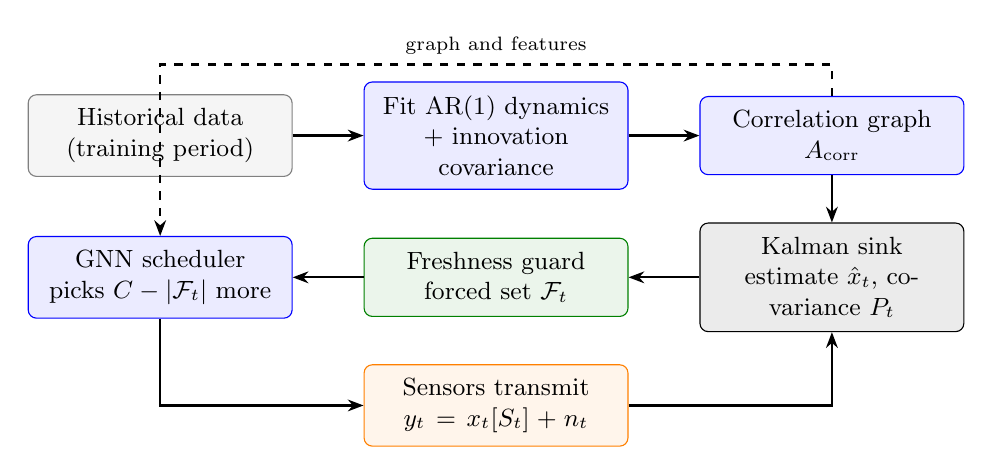
\begin{tikzpicture}[node distance=0.6cm and 0.9cm,
  box/.style={draw=#1,fill=#1!8,rounded corners=3pt,align=center,inner sep=5pt,font=\small,text width=3.0cm},
  box/.default=blue, arr/.style={-{Stealth[length=2mm]},thick}]
  \node[box=gray] (data) {Historical data\\(training period)};
  \node[box,right=of data] (fit) {Fit AR(1) dynamics\\ + innovation covariance};
  \node[box,right=of fit] (graph) {Correlation graph\\ $\Acorr$};
  \node[box=black,below=of graph] (sink) {Kalman sink\\ estimate $\hat x_t$, covariance $P_t$};
  \node[box=green!50!black,left=of sink] (guard) {Freshness guard\\ forced set $\mathcal F_t$};
  \node[box,left=of guard] (gnn) {GNN scheduler\\ picks $C-|\mathcal F_t|$ more};
  \node[box=orange,below=of guard] (net) {Sensors transmit\\ $y_t = x_t[S_t]+n_t$};
  \draw[arr] (data)--(fit); \draw[arr] (fit)--(graph); \draw[arr] (graph)--(sink);
  \draw[arr] (sink)--(guard); \draw[arr] (guard)--(gnn);
  \draw[arr] (gnn) |- (net); \draw[arr] (net) -| (sink);
  \draw[arr,dashed] (graph.north) -- ++(0,0.4) -| node[pos=0.25,above,font=\scriptsize]{graph and features} (gnn.north);
\end{tikzpicture}
\caption{The complete pipeline. The model and graph are fitted once on training data; the loop at the bottom runs
every slot.}
\end{figure}

\subsection{System model}

\begin{itemize}
  \item $M$ sensors with fixed positions. Time is divided into slots $t=1,2,\dots$ (5 minutes on real data).
  \item In each slot the sink chooses a set $S_t$ of at most $C$ sensors (\textbf{capacity constraint}).
  \item Optionally, sensors closer than an \textbf{interference radius} cannot transmit in the same slot (used only in
        the synthetic interference study; real-data experiments have no interference).
  \item Polled sensors send their reading with a small measurement noise: $y_t = x_t[S_t] + n_t$,
        $n_t\sim\mathcal N(0,rI)$, $r=10^{-3}$.
  \item Every sensor's age must satisfy $a_i(t)\le F$ (\textbf{freshness constraint}).
  \item Slot timeline: (1) the field moves one step, (2) the sink predicts, (3) the freshness guard computes forced
        sensors, (4) the scheduler completes the poll set, (5) the polled sensors transmit, (6) the sink updates,
        ages are updated, and the error is measured.
\end{itemize}

\subsection{Field model and the synthetic simulator}

Readings are modelled as a stationary, first-order autoregressive process with correlated innovations:
\[
  x_t = \operatorname{diag}(\rho)\,x_{t-1} + w_t,\qquad w_t\sim\mathcal N(0,Q).
\]
$\rho_i\in[0,1)$ says how much of sensor $i$'s value carries over to the next slot (temporal correlation); the
off-diagonal entries of $Q$ say how the sensors' surprises move together (spatial correlation).

\textbf{Synthetic simulator.} To test on thousands of controlled layouts, \texttt{CorrelatedField} generates fields
with a known ground truth:
\begin{enumerate}
  \item Place $M$ sensors in the unit square: \emph{uniform} (spread evenly) or \emph{clustered} (around 2--7 random
        centres with spread 0.07).
  \item Spatial correlation by an RBF kernel: $\Sigma_{ij}=\exp\!\big(-\lVert p_i-p_j\rVert^2/(2\ell^2)\big)$, where
        $\ell$ (length scale, default 0.3) controls how far correlation reaches.
  \item Per-sensor speed $\rho_i = \bar\rho \pm$ spread (default $\bar\rho=0.9$).
  \item Innovations $Q = D\Sigma D$ with $D=\operatorname{diag}(\sqrt{1-\rho_i^2})$, so every sensor has unit variance.
        The stationary covariance is $P_{0,ij}=Q_{ij}/(1-\rho_i\rho_j)$.
\end{enumerate}
The \textbf{layout seed} (positions, $\Sigma$, $\rho$) and the \textbf{noise seed} are separate. This fixes the
mid-semester bug: the graph is always estimated on the same layout the scheduler runs on (a unit test checks the
estimated and true correlations agree with $r>0.95$). Every policy is evaluated on the \emph{identical} trajectory
(the field is rewound between policies), so differences come only from the scheduling.

\subsection{Fitting the model from data}

The sink is never told the true model; it fits one from data (\texttt{fit\_model}). Given a block of training
readings $x_1,\dots,x_T$ (standardised):
\begin{align*}
  \hat\rho_i &= \frac{\sum_t x_{t-1,i}\,x_{t,i}}{\sum_t x_{t-1,i}^2}\quad(\text{clipped to }[0,0.9995]),\\
  e_t &= x_t - \hat\rho \odot x_{t-1}\quad(\text{innovations}),\qquad
  \hat Q = \operatorname{cov}(e_t)+10^{-6}I,\qquad \hat P_0=\operatorname{cov}(x_t)+10^{-6}I.
\end{align*}
\begin{whybox}[Why one-step least squares?]
It is the maximum-likelihood fit of an AR(1) model and is cheap even for 325 sensors and months of data. We also tried
fitting the autocorrelation at longer lags; on the real datasets it made the sink 4--17$\times$ over-confident (its
reported uncertainty was far below its actual error), so one-step fitting was kept.
\end{whybox}
For synthetic layouts the sink fits on a \textbf{pilot phase} of 1000 slots in which it hears every sensor. For real
data it fits on the training period only.

\subsection{The correlation graph}

From $\hat Q$ we compute the innovation correlation $\hat r_{ij}=\hat Q_{ij}/\sqrt{\hat Q_{ii}\hat Q_{jj}}$ and keep
strong edges:
\[
  (\Acorr)_{ij} = |\hat r_{ij}|\cdot\mathbf 1\big[|\hat r_{ij}|\ge 0.3\big],\qquad (\Acorr)_{ii}=0.
\]
\begin{whybox}[Why innovations, not raw readings?]
Raw readings of almost all sensors are correlated simply because they share trends (every room warms during the day,
every freeway slows at rush hour). That would connect everything to everything. Innovations remove the predictable
part, so an edge means ``when one sensor is surprised, the other is surprised in the same way'': exactly the
information that lets the sink infer one from the other. The threshold 0.3 keeps meaningful edges and drops noise.
\end{whybox}

\subsection{The Kalman sink}

The sink holds a mean $m$ and covariance $P$:
\begin{align*}
  \textbf{Predict:}\quad & m^- = \rho\odot m,\qquad P^- = D_\rho P D_\rho + Q,\qquad D_\rho=\operatorname{diag}(\rho)\\
  \textbf{Update:}\quad & K = P^-_{:,S}\,\big(P^-_{SS}+rI\big)^{-1},\quad m = m^- + K\,(y - m^-_S),\quad
  P = P^- - K\,P^-_{S,:}
\end{align*}
Here $S$ is the set of polled sensors. Polling sensor $j$ reduces $P_{ii}$ for every $i$ with $P_{ij}\neq0$: the
correlated neighbours learn too (a unit test checks this). $P$ does not depend on the actual readings, only on
\emph{who} was polled, so the scheduler can plan with it.

\textbf{Variance gain.} If sensor $i$ alone were polled next, the total uncertainty would drop by
\[
  g_i = \frac{\sum_k P_{ki}^2}{P_{ii}+r}.
\]
This single number drives the Kalman-greedy baseline and the first term of our decoder.

\begin{whybox}[Why a Kalman filter, not a neural forecaster?]
It is optimal for the linear-Gaussian model, needs no training, gives a calibrated uncertainty $P$ (a unit test
checks that the predicted variance matches the actual error within 8\%), and updates in milliseconds. A learned
forecaster would not give us $P$, which is what makes correlation-aware scheduling possible.
\end{whybox}

\subsection{The freshness guard}

Before any scheduler acts:
\begin{enumerate}
  \item Find all sensors with $a_i(t)\ge F$.
  \item Sort them oldest first and take up to $C$ of them that do not conflict with each other: this is the forced
        set $\mathcal F_t$.
  \item The scheduler only fills the remaining $C-|\mathcal F_t|$ places.
  \item The environment checks (asserts) in every slot that capacity, conflicts and freshness hold.
\end{enumerate}
We use $F=\lfloor 3M/C\rfloor$: three times the round-robin period. Intel: $F=\lfloor 3\cdot45/6\rfloor=22$ slots
(1.8 hours). PEMS-BAY: $F=\lfloor3\cdot325/40\rfloor=24$ slots (2 hours). Synthetic headline: $F=15$.

\begin{whybox}[Why a hard guard instead of a penalty in the reward?]
A penalty can always be traded away: if ignoring a sensor reduces error enough, the policy will ignore it. A guard
makes the guarantee unconditional and identical for every scheduler, which also makes comparisons fair.
Section 8 shows what happens without it: Kalman-greedy never polls 18 of 50 sensors.
\end{whybox}

\begin{whybox}[Why $F = 3M/C$?]
Round robin needs $M/C$ slots to visit everyone. A bound equal to $M/C$ would force pure round robin and leave no
freedom; a very large bound would allow near-starvation. Three times the period gives the scheduler real freedom
while still keeping every sensor within a couple of hours on real data.
\end{whybox}

\subsection{Objective and MDP formulation}

\textbf{Objective.}
\[
  \min_\pi\ \mathbb E\Big[\frac{1}{TM}\sum_{t=1}^T\lVert x_t-\hat x_t\rVert^2\Big]
  \quad\text{s.t.}\quad |S_t|\le C,\ \text{no conflicts in } S_t,\ a_i(t)\le F\ \ \forall i,t.
\]

\textbf{As an MDP:}
\begin{itemize}
  \item \textbf{State}: ages $a(t)$, which sensors were polled last slot, the sink's covariance $P_t$, the learned
        $\hat\rho$ and graph $\Acorr$, the conflict matrix, the forced set.
  \item \textbf{Action}: an ordered list of $C-|\mathcal F_t|$ sensors to poll.
  \item \textbf{Transition}: the field evolves, the sink predicts and updates, ages change.
  \item \textbf{Reward}: $r_t = -(1-\gamma)\log(\text{error}_t + 0.005)$ (details in 5.9).
\end{itemize}

\subsection{The GNN scheduler}

\subsubsection{Node features (13 per sensor)}
\begin{center}
\small
\begin{tabularx}{\textwidth}{@{}rlX@{}}
\toprule
\# & Feature & Why it is there \\
\midrule
1 & $\min(a_i/(M/C),6)/6$ & Age relative to the round-robin period (comparable across network sizes) \\
2 & polled last slot (0/1) & Recently polled sensors usually need no repeat \\
3 & $P_{ii}$ & The sink's uncertainty about sensor $i$ \\
4 & $\log(P_{ii}+10^{-3})/7$ & Same on a log scale (uncertainty spans orders of magnitude) \\
5 & $g_i/M$ & How much total uncertainty polling $i$ removes \\
6 & $\log(g_i/M+10^{-4})/9$ & Same on a log scale \\
7 & forced (0/1) & Already committed by the guard \\
8 & slack $=\mathrm{clip}((F-a_i)/F,0,1)$ & How soon the guard will force this sensor \\
9 & $C/M$ & How scarce the channel is \\
10 & $\hat\rho_i$ & How persistent the sensor is \\
11 & $\log(1-\hat\rho_i^2+10^{-5})/12$ & How fast it drifts away from its last value \\
12 & degree in $\Acorr$ / $(M-1)$ & How connected (redundant) it is \\
13 & guard on (0/1) & Whether a freshness bound applies \\
\bottomrule
\end{tabularx}
\end{center}
All features are scaled to roughly $[0,1]$ so one network works across network sizes.

\subsubsection{Two graphs}
\begin{itemize}
  \item $\Acorr$: the static correlation graph (who is correlated in general).
  \item $\Apost$ with $(\Apost)_{ij}=|P_{ij}|/\sqrt{P_{ii}P_{jj}}$: the sink's \emph{current} posterior correlation,
        recomputed every slot (who is redundant \emph{right now}, given what was just polled).
\end{itemize}
Both are row-normalised ($\tilde A = A/\text{row sum}$) before use.

\subsubsection{Encoder}
\begin{align*}
  h^{(0)}_i &= \mathrm{MLP}_{\text{in}}(\text{features}_i)\in\mathbb R^{64}\\
  h^{(\ell+1)} &= \mathrm{LN}\Big(h^{(\ell)} + \mathrm{MLP}_\ell\big[\,h^{(\ell)},\ \tilde\Acorr h^{(\ell)},\ \tilde\Apost h^{(\ell)},\ \bar h^{(\ell)}\,\big]\Big),\quad \ell=0,1,2
\end{align*}
$\bar h$ is the mean over all sensors (global context). Each MLP is $4d\to2d\to d$ with GELU. Three layers let
information travel three hops. The residual connection and LayerNorm keep training stable.

\subsubsection{Residual pointer decoder}
Sensors are picked one at a time. At each step the score (logit) of sensor $i$ is
\[
  \text{logit}_i = \underbrace{\alpha\log g_i}_{\text{Kalman-greedy}} + \underbrace{f_\theta(h_i)}_{\text{learned correction}}
  + \underbrace{\textstyle\sum_{j\in\text{picked}} G_{ij}}_{\text{learned interaction}},\qquad G_{ij}=\frac{q_i^\top k_j}{\sqrt{32}}.
\]
\begin{enumerate}
  \item Mask sensors already picked, forced, or in conflict with a pick.
  \item Softmax over the remaining scores; \emph{sample} a sensor during training, take the \emph{argmax} at test time.
  \item Condition $P$ on that pick (Kalman update), recompute every $g_i$, add $G_{\cdot,\text{pick}}$.
  \item Repeat until the slot is full.
\end{enumerate}

\textbf{Residual initialisation.} The output layers of $f_\theta$ and $q$ are initialised to zero, so at the start
$f_\theta=G=0$ and the decoder \emph{is} Kalman-greedy (with $\alpha=4$ the softmax is sharp). A unit test checks that
the untrained network makes exactly the same choices as Kalman-greedy for 40 slots.

\textbf{Plackett--Luce probability.} The probability of the ordered pick list is the product of the softmax
probabilities at each step, so PPO gets exact log-probabilities (also unit-tested).

Size: 137{,}282 parameters. The same weights run for any $M$.

\begin{whybox}[Why a residual decoder?]
Our first attempt trained a GNN ``student'' to imitate Kalman-greedy (behaviour cloning) and then fine-tune; it never
fully matched the teacher. Building Kalman-greedy \emph{into} the network means training starts from the strongest
model-based scheduler, and RL only has to learn \emph{when deviating from greedy pays off later}, for example polling a
sensor before the guard forces it at a bad moment, or not trusting a wrong model.
\end{whybox}

\subsection{Training with PPO}

\begin{algorithm}[htbp]
\caption{PPO training of the GNN scheduler}
\begin{algorithmic}[1]
\State Actor $\pi_\theta$ = Kalman-greedy at init; critic $V_\phi$ (2-layer GNN)
\For{iteration $=1..400$}
  \State Sample a batch of environments: synthetic (random $M\in[10,100]$, $C$, $\ell$, $\rho$, layout, $F$, interference)
  \Statex\hspace{1.3em}or, with probability 0.35, replays of a real dataset's training period
  \For{$t=1..96$ slots}
    \State $\mathcal F_t\gets$ guard; sample picks from $\pi_\theta$; step; reward $r_t=-(1-\gamma)\log(\text{err}_t+0.005)$
  \EndFor
  \State Advantages with GAE ($\gamma=0.95$, $\lambda=0.9$)
  \For{4 epochs over minibatches of 512}
    \State ratio $\eta=\pi_\theta/\pi_{\text{old}}$; loss $-\min(\eta\hat A,\ \mathrm{clip}(\eta,0.85,1.15)\hat A) - 0.002\cdot\text{entropy}$
    \State Adam step (lr $10^{-4}$ actor, $5\times10^{-4}$ critic, grad-norm clip 0.5)
  \EndFor
  \State Every 10 iterations: validate, keep the best checkpoint
\EndFor
\end{algorithmic}
\end{algorithm}

\textbf{Training scenarios.} Each synthetic batch draws: $C=\mathrm{round}(M\cdot U[0.08,0.35])$; length scale
log-uniform in $[0.05,0.45]$; $\bar\rho\in U[0.6,0.995]$; per-sensor spread with probability 0.6; clustered layout with
probability 0.4; freshness bound $3M/C$ with probability 0.7 (else off); interference with probability 0.2. The
number of parallel environments shrinks for large $M$ ($32\cdot(40/M)^2$, clipped to 8--32) to keep memory constant.

\textbf{Reward.} For synthetic environments the score is the sink's true posterior variance (computed with the true
model); for real replays it is the actual squared error against the recorded readings. The logarithm puts small
networks (large errors) and large networks (small errors) on the same scale, and the $(1-\gamma)$ factor keeps
returns near the reward scale.

\textbf{Real-data replays.} On a real dataset's training period, the sink's model is fitted on the first 70\%, the
episodes run on the next 20\% (on compact sub-networks: a random sensor and its nearest neighbours), and the last
10\% is validation. Because the model is fitted on different days than the episode, the policy experiences the
model mismatch it will face at test time.

\textbf{Validation and selection.} Validation uses four fixed synthetic scenarios (default $M=20,C=5,F=12$;
clustered; heterogeneous $\rho$; $M=60,C=8,F=22,\ell=0.15$) with layout seeds 9000+, plus real validation slices.
The checkpoint with the best validation score is kept. Test layouts use seeds 10000+ and real test periods; neither
is ever seen in training.

\textbf{Run.} 400 PPO iterations (resumable; warm-started from an earlier run), about 35 minutes on a laptop CPU.
The critic is warmed up for 15 iterations before the actor starts updating.

\subsection{Baselines and evaluation protocol}

\begin{center}
\small
\begin{tabularx}{\textwidth}{@{}lX@{}}
\toprule
\textbf{Scheduler} & \textbf{Rule (after the forced sensors)} \\
\midrule
Random & Pick uniformly at random. Lower reference. \\
Max-AoI (B1) & Pick the oldest sensors (ties by index, so round robin). AoI-based scheduling \cite{2,16}. \\
Corr-diverse (v4) & Pick the oldest; then multiply every other sensor's score by $(1-|\hat r|)$ with the picked one; repeat. Our mid-semester heuristic. \\
Max-uncertainty & Pick the largest $P_{ii}$, ignoring overlap between picks. \\
Kalman-greedy & Repeatedly pick the largest $g_i$ and condition $P$ on it \cite{19}. Strongest model-based baseline. \\
Oracle-greedy & Kalman-greedy using the \emph{true} covariance (synthetic only; not deployable). \\
GNN-PPO (ours) & Learned policy (greedy decode). \\
Ablation & Our model retrained with the message passing removed. \\
\bottomrule
\end{tabularx}
\end{center}

\textbf{Metrics.}
\begin{itemize}
  \item \textbf{MSE}: mean over sensors and slots of $(x-\hat x)^2$ in standardised units.
  \item \textbf{RMSE in units}: the same error converted back to $^\circ$C or mph (what the faculty can relate to).
  \item \textbf{Mean AoI} and \textbf{max AoI}; \textbf{starved} = number of sensors never polled.
  \item \textbf{Decision time} per slot (milliseconds on CPU).
\end{itemize}
The first 50 slots of each synthetic episode are burn-in and not scored.

\textbf{Statistics.} Mean $\pm$ 95\% CI ($1.96\cdot\text{sd}/\sqrt n$) over test layouts or windows. Because every
scheduler runs on the identical readings, we compare them \emph{paired}: the \textbf{win rate} is the share of
windows where the GNN had lower error, and the \textbf{Wilcoxon signed-rank test} gives the p-value.

\section{Implementation, step by step}

This is the order in which the project was actually built.

\subsection{Step 1: Review the mid-semester prototype}
The prototype (now in \texttt{legacy/}) used 5 sensors and random data. Reviewing it, we found the seed bug: the
correlation graph was estimated on layout seed 42 but the scheduler was evaluated on seed 123. Because the seed also
placed the sensors, the graph described a different set of sensors (correlation $r=0.04$ with the truth). Decision:
rebuild as a clean, tested Python package and keep the legacy code only for reference.

\subsection{Step 2: Simulator, environment and Kalman sink}
\begin{itemize}
  \item \texttt{config.py}: one \texttt{Scenario} object holds every setting ($M$, $C$, length scale, $\rho$, layout,
        noise, interference, pilot length, graph threshold, freshness bound).
  \item \texttt{simulator.py}: the correlated field (Section 5.2), with separate layout and noise seeds, and
        \texttt{fit\_model}.
  \item \texttt{graphs.py}: correlation and interference graphs.
  \item \texttt{estimator.py}: the Kalman sink.
  \item \texttt{env.py}: the slot loop, ages, the freshness guard and safety assertions, and per-slot metrics. It can
        \emph{rewind} the field so every policy sees identical readings.
\end{itemize}
Tests written at this stage: the field has the target covariance, the graph matches the sensors it is used on, the
Kalman variance is calibrated, polling reduces neighbours' uncertainty.

\subsection{Step 3: Baselines and the evaluation harness}
\texttt{policies/baselines.py} implements the five baselines and the oracle; \texttt{selection.py} has the shared
greedy and feasibility routines; \texttt{evaluate.py} runs episodes in parallel across CPU cores and summarises
metrics with confidence intervals. A parametrised test runs every baseline and checks it never breaks freshness,
capacity or interference.

\subsection{Step 4: The GNN and how its design evolved}
\begin{enumerate}
  \item First version: a GNN that scored sensors, trained by behaviour cloning on Kalman-greedy's choices. It
        under-performed its own teacher.
  \item Final version: the residual pointer decoder (Section 5.8). It starts as Kalman-greedy exactly, so learning only
        has to add improvements.
\end{enumerate}
Files: \texttt{gnn/features.py} (13 features, two graphs, batching), \texttt{gnn/model.py} (encoder, decoder, critic),
\texttt{policies/gnn\_policy.py} (wraps the model as a scheduler).

\subsection{Step 5: PPO training}
\texttt{gnn/train.py} implements Algorithm~1. Two engineering fixes mattered:
\begin{itemize}
  \item \textbf{Environment reset bug}: resetting an environment did not rewind the field, so rollouts and evaluation
        saw different readings. Fixed with \texttt{mark()}/\texttt{rewind()} and a regression test.
  \item \textbf{Long runs killed}: training stopped when the terminal session closed. We made training
        \textbf{resumable} (state saved regularly) and ran it detached; the final run was warm-started from an
        earlier checkpoint.
\end{itemize}

\subsection{Step 6: Real datasets}
Following our faculty's request for more sensors and real data, \texttt{datasets.py} adds two datasets.

\textbf{Intel Berkeley Research Lab} \cite{25}.
\begin{enumerate}
  \item Raw data: 54 Mica2Dot motes, temperature about every 31 seconds, plus mote positions in metres on a
        40\,m $\times$ 31\,m floor.
  \item Keep readings between 5 and 45\,$^\circ$C (removes sensor faults), from 28 Feb 2004 01:00 to 19 Mar 2004 (after
        that, batteries die and data degrades).
  \item Average into 5-minute slots.
  \item Keep motes with at least 70\% of slots present; fill gaps up to 2 hours (24 slots) by interpolation; drop
        motes still incomplete. Result: \textbf{45 sensors}.
  \item Chronological split: first 55\% for training (28 Feb -- 8 Mar), the rest for testing (9 -- 18 Mar).
  \item The recording has \textbf{outages} (network down, e.g.\ 10--11 and 15--16 Mar). We record where each continuous
        segment ends; test windows never cross a gap, and a live session stops cleanly at one (tested).
\end{enumerate}

\textbf{PEMS-BAY} \cite{24}.
\begin{enumerate}
  \item 325 loop detectors in the San Jose area, average speed every 5 minutes, 1 Jan -- 30 Jun 2017 (public release
        accompanying DCRNN, Zenodo record 5146275).
  \item Zero speeds mark missing data; they are interpolated.
  \item Training: January--April. Test: May--June.
\end{enumerate}

\textbf{Common preprocessing.}
\begin{itemize}
  \item \textbf{Daily profile}: for every 5-minute time of day (and for PEMS-BAY separately for weekdays and weekends),
        the average reading over the training period, smoothed over 5 neighbouring bins. The sink knows that ``rush
        hour happens''; what it must track is how \emph{today} differs from a typical day.
  \item \textbf{Standardise} the deviation from the profile by its training standard deviation.
  \item All statistics come from the training period only; a test checks that the test period never leaks into the
        model and that replayed readings match the raw data exactly.
  \item Memory: float32 storage, chunked computation, a small profile table, and pre-fitted model files reduced memory
        from about 1.75\,GB to 200--400\,MB.
\end{itemize}

\textbf{Test windows.} Intel: 10 disjoint windows of 200 slots in the test period. PEMS-BAY: 15 windows of 288 slots
(one day each). Capacity $C=6$ (Intel) and $C=40$ (PEMS-BAY), about one-eighth of the sensors.

\subsection{Step 7: Experiments and figures}
\texttt{experiments.py} runs every study and writes JSON to \texttt{results/data/}; \texttt{viz/} draws the figures in
\texttt{results/figures/}:
\begin{itemize}
  \item synthetic main benchmark (30 layouts, uniform and clustered), no-guard study, capacity / correlation / size /
        interference / pilot-length sweeps;
  \item real benchmark, real capacity sweeps, PEMS-BAY size sweep, poll-frequency map, slot-by-slot replay;
  \item significance tests and decision times.
\end{itemize}

\subsection{Step 8: Live demo}
\begin{itemize}
  \item \texttt{live.py}: a \texttt{LiveSession} replays a real test day slot by slot and runs several schedulers on
        identical readings. Each step returns the readings, each scheduler's picks (forced ones marked), the GNN's pick
        probabilities, and the sink's estimates and uncertainties.
  \item \texttt{server.py}: a small HTTP server with a JSON API: \texttt{/api/datasets}, \texttt{/api/session},
        \texttt{/api/step}, \texttt{/api/results}, \texttt{/health}.
  \item \texttt{frontend/}: plain HTML/CSS/JavaScript with Canvas: the measured field and each scheduler's view of it,
        the error over time, ``why these sensors'' bars, and a transmission log.
\end{itemize}

\subsection{Step 9: Testing, CI and release}
21 tests (\texttt{tests/test\_core.py}) run on every push with GitHub Actions. The repository is public:
\texttt{github.com/BhanuPrasadPalella-01/gnn-aoi-scheduler}.

\subsection{Code map and commands}
\begin{center}
\small
\begin{tabularx}{\textwidth}{@{}lX@{}}
\toprule
\texttt{gnn\_aoi/config.py} & Scenario settings \\
\texttt{gnn\_aoi/simulator.py} & Synthetic field, AR(1) model, \texttt{fit\_model} \\
\texttt{gnn\_aoi/datasets.py} & Intel Lab and PEMS-BAY loaders, profiles, outages, test windows \\
\texttt{gnn\_aoi/graphs.py} & Correlation and interference graphs \\
\texttt{gnn\_aoi/estimator.py} & Kalman sink \\
\texttt{gnn\_aoi/env.py} & Slot loop, AoI, freshness guard, metrics \\
\texttt{gnn\_aoi/selection.py} & Greedy variance reduction, feasible top-$C$ \\
\texttt{gnn\_aoi/policies/} & Baselines and the GNN policy \\
\texttt{gnn\_aoi/gnn/} & Features, model, PPO training \\
\texttt{gnn\_aoi/evaluate.py}, \texttt{experiments.py} & Benchmarks, sweeps, statistics \\
\texttt{gnn\_aoi/live.py}, \texttt{server.py}, \texttt{frontend/} & Live demo \\
\texttt{gnn\_aoi/viz/} & Figures and animation \\
\texttt{tests/} & 21 tests \\
\bottomrule
\end{tabularx}
\end{center}

\begin{center}
\small
\begin{tabular}{@{}ll@{}}
\toprule
\texttt{python -m gnn\_aoi download} & fetch the raw datasets \\
\texttt{python -m gnn\_aoi train} & train the GNN with PPO \\
\texttt{python -m gnn\_aoi experiments} & run all experiments \\
\texttt{python -m gnn\_aoi figures} & draw all figures \\
\texttt{python -m gnn\_aoi serve} & live demo at \texttt{http://localhost:8000} \\
\texttt{python -m pytest} & run the tests \\
\bottomrule
\end{tabular}
\end{center}

\section{Design decisions: why this, and why not that}

\subsection{Datasets}

\begin{whybox}[Why the Intel Berkeley Research Lab dataset?]
\begin{itemize}
  \item It is a \textbf{real wireless sensor network}: battery motes on one floor reporting to a base station, the
        exact setting of our problem.
  \item The motes' \textbf{positions are published}, so we can draw the network and check that learned correlations
        make physical sense.
  \item Indoor temperature is \textbf{strongly spatially correlated} (rooms, corridors, sun-facing walls): the
        case where correlation-aware scheduling should help most.
  \item It is public, widely used in sensor-network research, and small enough to run on a laptop.
\end{itemize}
\end{whybox}

\begin{whybox}[Why PEMS-BAY as the second dataset?]
\begin{itemize}
  \item \textbf{Scale}: 325 sensors, seven times more than Intel. It tests whether the method scales.
  \item \textbf{Different physics}: traffic speed changes suddenly (incidents, congestion waves) and correlation
        follows the road network, not straight-line distance. A good test of robustness.
  \item \textbf{Clean and long}: six months of 5-minute data with few gaps, so we can train on four months and test
        on two.
  \item It is a \textbf{standard benchmark} in spatio-temporal graph learning (introduced with DCRNN \cite{24}).
\end{itemize}
\end{whybox}

\textbf{Why not the alternatives?}
\begin{itemize}
  \item \textbf{Random / synthetic data only}: exactly what the faculty asked us to move away from. We keep the
        simulator for controlled studies, but the headline results are on real data.
  \item \textbf{METR-LA} (207 Los Angeles traffic sensors): same type of data as PEMS-BAY but with many more missing
        readings; PEMS-BAY is cleaner and larger.
  \item \textbf{Single-station datasets} (e.g.\ one air-quality or weather station): no spatial network, so there is
        no correlation between sensors to exploit.
  \item \textbf{Sparse weather or pollution networks}: stations kilometres apart, hourly data and many gaps; weak
        correlation and too few slots.
  \item \textbf{Private or paid datasets}: not reproducible.
\end{itemize}
Using one indoor dataset with strong correlation and one large outdoor dataset with weaker, more irregular
correlation shows both where the method helps a lot and where it helps a little.

\subsection{Problem settings}

\begin{whybox}[Why 5-minute slots?]
It is PEMS-BAY's native resolution, and Intel's 31-second readings average cleanly into it. It also matches how often
a battery sensor would realistically report.
\end{whybox}
\begin{whybox}[Why $C\approx M/8$ (6 of 45, 40 of 325)?]
Capacity must be scarce for scheduling to matter; with $C$ close to $M$ every scheduler polls almost everyone. About one
in eight is a realistic shared-channel budget, and the capacity sweeps show results for $C$ from 3 to 15 (Intel) and
10 to 80 (PEMS-BAY).
\end{whybox}
\begin{whybox}[Why a correlation threshold of 0.3?]
Below about 0.3, sample correlations are dominated by estimation noise and would add many meaningless edges; much higher
thresholds would drop real relationships. The Kalman filter still uses the full covariance; the threshold only shapes
the graph the GNN passes messages on.
\end{whybox}

\subsection{Algorithms}

\textbf{Estimator: Kalman filter.} Alternatives: particle filters (needed only for non-Gaussian models, much slower),
Gaussian-process regression (no time dynamics, cubic cost per slot), deep forecasters such as graph-recurrent networks
(need training, no calibrated uncertainty). The Kalman filter is optimal for our model, fast, and its covariance is
exactly the uncertainty signal the scheduler needs.

\textbf{Learning paradigm: reinforcement learning.} Supervised learning needs the ``right'' poll set for every slot,
which nobody knows: a choice now affects errors and forced polls many slots later. RL learns from the outcome itself.

\textbf{RL algorithm: PPO.}
\begin{itemize}
  \item \textbf{DQN} needs a value for every possible action. Choosing 6 of 45 sensors has over 8 million combinations
        (40 of 325 is astronomically more); a Q-network cannot enumerate them. Our pointer decoder builds the set one
        sensor at a time with exact probabilities, which suits policy-gradient methods.
  \item \textbf{REINFORCE / A2C}: simpler policy gradients, but with high variance and unstable large updates; PPO's
        clipping makes training stable.
  \item \textbf{SAC / DDPG}: designed for continuous actions; ours are discrete selections.
  \item PPO is the most widely used, robust on-policy algorithm and easy to tune.
\end{itemize}

\textbf{Model: graph neural network.}
\begin{itemize}
  \item \textbf{MLP}: fixed input size, so a model for 45 sensors cannot run on 325, and it would have to learn that
        sensor order does not matter.
  \item \textbf{CNN}: needs a regular grid; sensors are irregularly placed and traffic follows roads.
  \item \textbf{Transformer}: also permutation-equivariant, but attends from every sensor to every other ($M^2$
        attention) and ignores the known correlation structure. A GNN uses the graph we already learned. (Our decoder
        does use a light query--key interaction term.)
\end{itemize}

\textbf{Decoder: residual pointer network.} Scoring all sensors once and taking the top $C$ ignores that the second pick
should depend on the first (two neighbours are redundant). The autoregressive pointer decoder \cite{22} re-scores after
each pick and re-runs the Kalman update, so redundancy is handled exactly. Starting from Kalman-greedy (instead of a
random initialisation or behaviour cloning) gives a strong policy from iteration 0.

\textbf{Freshness: hard guard, not a penalty or probabilistic constraint.} Explained in Section 5.6: unconditional,
identical for all policies, and the only way to guarantee no starvation.

\textbf{Statistics: Wilcoxon signed-rank test.} The same windows are used for every scheduler, so the results are
paired. A paired t-test assumes normally distributed differences; with 10--30 samples and skewed errors, Wilcoxon (which
uses ranks) is the safer choice.

\subsection{Tools}

\begin{center}
\small
\begin{tabularx}{\textwidth}{@{}p{3.3cm}p{3.3cm}X@{}}
\toprule
\textbf{Chosen} & \textbf{Instead of} & \textbf{Reason} \\
\midrule
Python & MATLAB, Java & Standard language for ML; free; all libraries available. \\
NumPy & Pandas for core maths & Fast vectorised linear algebra for the Kalman filter; Pandas used only to parse raw files. \\
PyTorch & TensorFlow, JAX & Dynamic graphs make the step-by-step decoder easy; dominant in research; good CPU performance. \\
Dense matrices for message passing & PyTorch Geometric, DGL & With $M\le325$, one batched matrix multiply is faster and simpler than sparse scatter operations, and avoids a heavy, version-sensitive dependency. \\
CPU training & GPU & The model is small (137k parameters); the Kalman steps are sequential; 35 minutes on a laptop CPU is enough, and anyone can reproduce it. \\
Matplotlib & Plotly, Seaborn & Publication-quality static figures and the GIF, no extra dependencies. \\
Python standard-library HTTP server & Flask, FastAPI, Django & Five small JSON endpoints; zero extra dependencies; runs anywhere Python runs. \\
Plain JavaScript + Canvas & React, D3 & No build step; Canvas draws hundreds of animated sensors smoothly. \\
pytest + GitHub Actions & Manual testing & Every push re-checks guarantees such as freshness and no data leakage. \\
LaTeX Beamer & PowerPoint & Required by the review; equations and references typeset properly. \\
\bottomrule
\end{tabularx}
\end{center}

\subsection{Hyper-parameters}
\begin{itemize}
  \item \textbf{Embedding 64, 3 layers}: information reaches three-hop neighbourhoods while the model stays small
        (137k parameters) and fast on a CPU.
  \item \textbf{$\gamma=0.95$}: about a 20-slot horizon, similar to the freshness bound, so the policy can plan around
        forced polls.
  \item \textbf{Clip 0.15, lr $10^{-4}$}: small steps, because the policy starts already strong (Kalman-greedy) and
        large updates would destroy that.
  \item \textbf{Entropy 0.002}: a little exploration without making the policy noisy.
  \item \textbf{35\% real-data iterations}: enough to learn real-world mismatch while synthetic variety teaches
        generalisation.
\end{itemize}

\section{Results: expected output, obtained output, and every graph explained}

\subsection{What we expected}
Before running the final experiments we expected:
\begin{enumerate}[label=\textbf{E\arabic*}]
  \item Correlation-aware schedulers (Kalman-greedy, the GNN) would clearly beat Max-AoI wherever sensors are
        correlated, with the same freshness guarantee.
  \item The gain would grow with correlation strength and disappear when sensors are independent.
  \item The GNN would at least match Kalman-greedy (it starts as Kalman-greedy) and beat it where looking ahead or
        robustness to a wrong model matters, especially on real data.
  \item Without the freshness guard, greedy schedulers would neglect some sensors entirely.
  \item The scheduler would be fast enough for real time: well under the 5-minute slot.
\end{enumerate}

\subsection{What we obtained (summary)}
\begin{center}
\small
\begin{tabularx}{\textwidth}{@{}lXl@{}}
\toprule
& \textbf{Obtained} & \textbf{Verdict} \\
\midrule
E1 & Synthetic: about 50\% (uniform) and 69\% (clustered) lower MSE than Max-AoI. Intel: 20\% lower RMSE. PEMS-BAY: 2.4\%. & Confirmed; much larger indoors \\
E2 & Gain $\approx$3\% at length scale 0.05, $\approx$68\% at 0.45. & Confirmed \\
E3 & GNN beats Kalman-greedy in 10/10 Intel and 15/15 PEMS-BAY windows; 73\% of synthetic layouts; ties on clustered layouts. Kalman-greedy is better on synthetic networks of 100+ sensors. & Mostly confirmed \\
E4 & Without the guard Kalman-greedy never polls 18 of 50 sensors; the GNN polls all of them. & Confirmed \\
E5 & 4.6\,ms (Intel), 37\,ms (PEMS-BAY) per slot vs.\ a 300-second slot. & Confirmed \\
\bottomrule
\end{tabularx}
\end{center}

Unexpected findings: (i) on real data, the model \emph{without message passing} matches the full GNN; (ii) on
PEMS-BAY, Kalman-greedy is \emph{worse} than plain Max-AoI because its fitted model is over-confident; (iii) the GNN
beats even the oracle that knows the true covariance on synthetic data.

\subsection{How to read the figures}
All figures use the same colours: \textbf{blue} = GNN-PPO (ours), \textbf{orange-red} = Max-AoI (B1),
\textbf{teal} = Kalman-greedy, \textbf{gold} = Corr-diverse (v4), \textbf{pink} = oracle-greedy or the ablation (dotted),
\textbf{green} = max-uncertainty, \textbf{purple} = random. Error bars and shaded bands are 95\% confidence intervals:
if two bands do not overlap, the difference is clearly real. ``Lower is better'' for every error axis.

%-------------------------------------------------------------------------------
\subsection{Figure: live scheduling on real data (the hero figure)}
\begin{figure}[H]\centering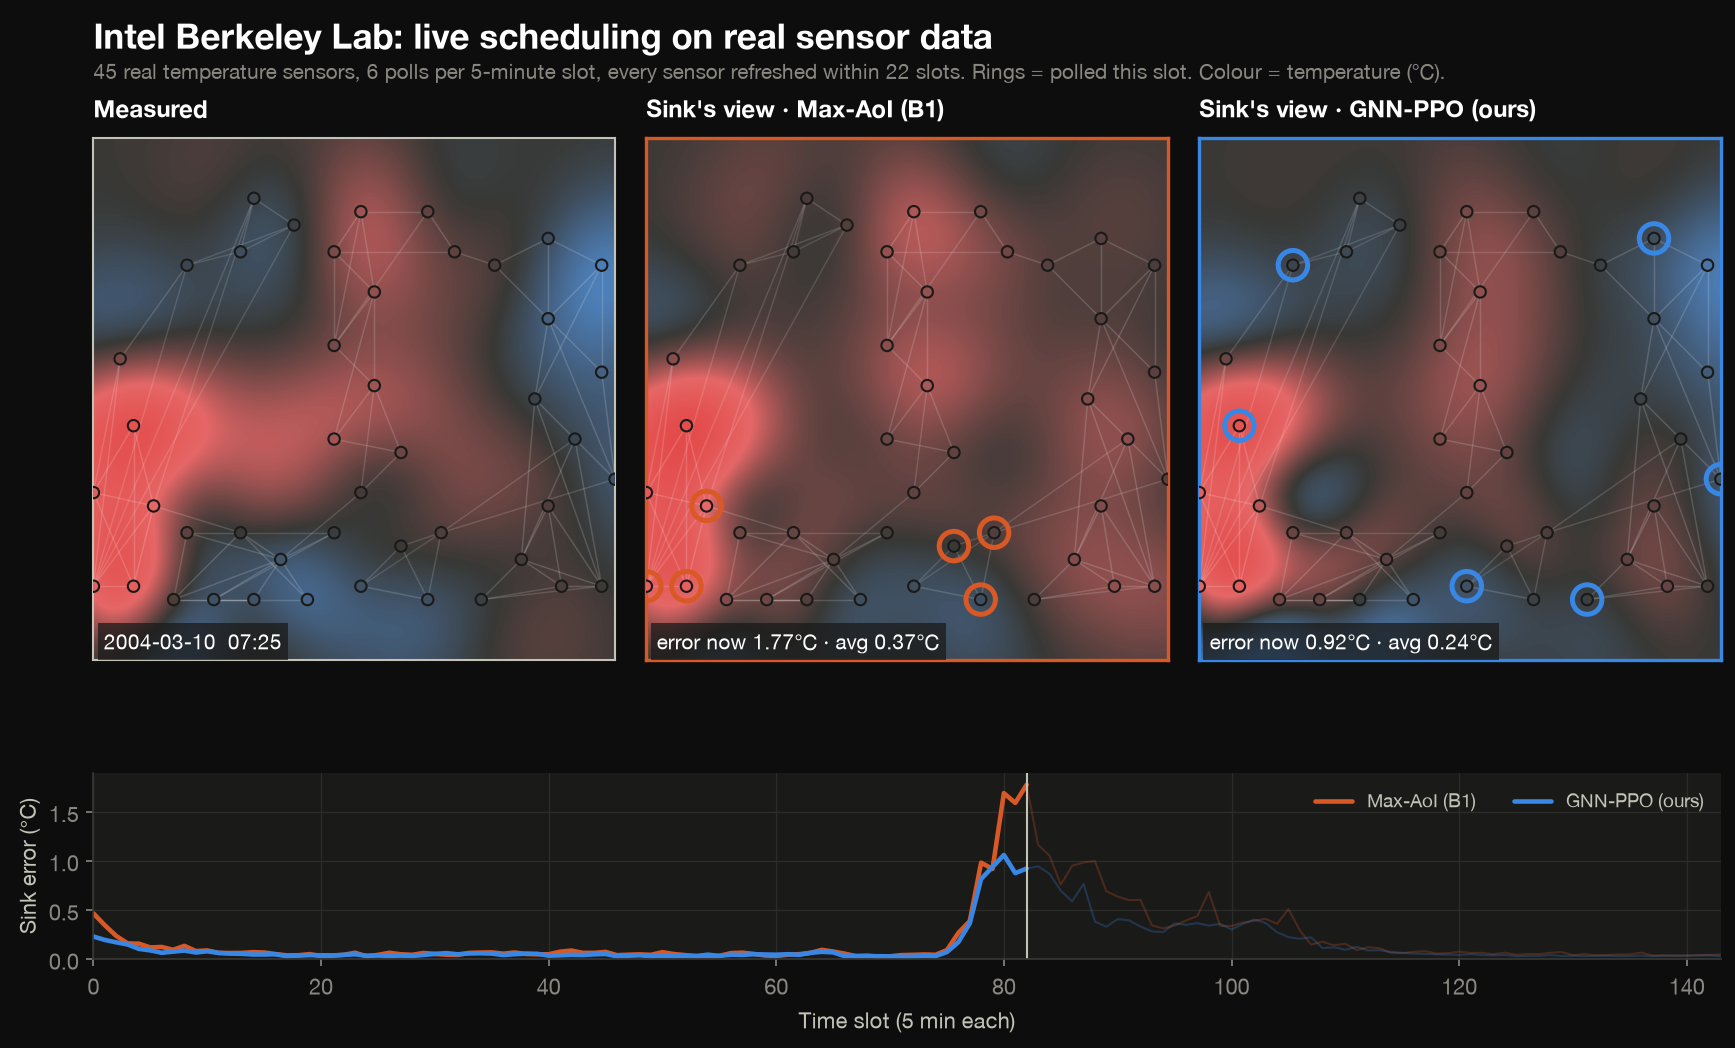
\includegraphics[width=\textwidth]{hero.png}
\caption{Intel Lab, one moment of a replay: the measured field and the sink's view under Max-AoI and under the GNN.}\end{figure}

\textbf{What is shown.} Three maps of the lab floor at 10 March 2004, 07:25. Colour is temperature (blue cool, red
warm). Left: the measured readings. Middle and right: what the sink \emph{believes} the floor looks like under
Max-AoI and under our GNN. Circles with rings are the sensors polled in this slot; thin lines are correlation-graph
edges. The bottom panel is the sink's error over 144 slots (12 hours).

\textbf{What it shows.} Around slots 75--85 the temperatures change quickly. Max-AoI's error
spikes to about 1.8\,$^\circ$C because it keeps polling sensors in fixed rotation; the GNN's spike stays near 1\,$^\circ$C because it
polls sensors spread across regions that are changing. Averages over the whole replay: 0.37\,$^\circ$C (Max-AoI) vs.\ 0.24\,$^\circ$C (GNN).

\begin{saybox}
``Left is reality, the other two are what the base station thinks. When the lab suddenly warms up, the classic
scheduler is still polling sensors in turn, so its picture goes wrong by almost 2 degrees. Our scheduler spends its
six transmissions on sensors that cover the changing areas, so its picture stays close to reality.''
\end{saybox}

%-------------------------------------------------------------------------------
\subsection{Figure: real-data benchmark (main result)}
\begin{figure}[H]\centering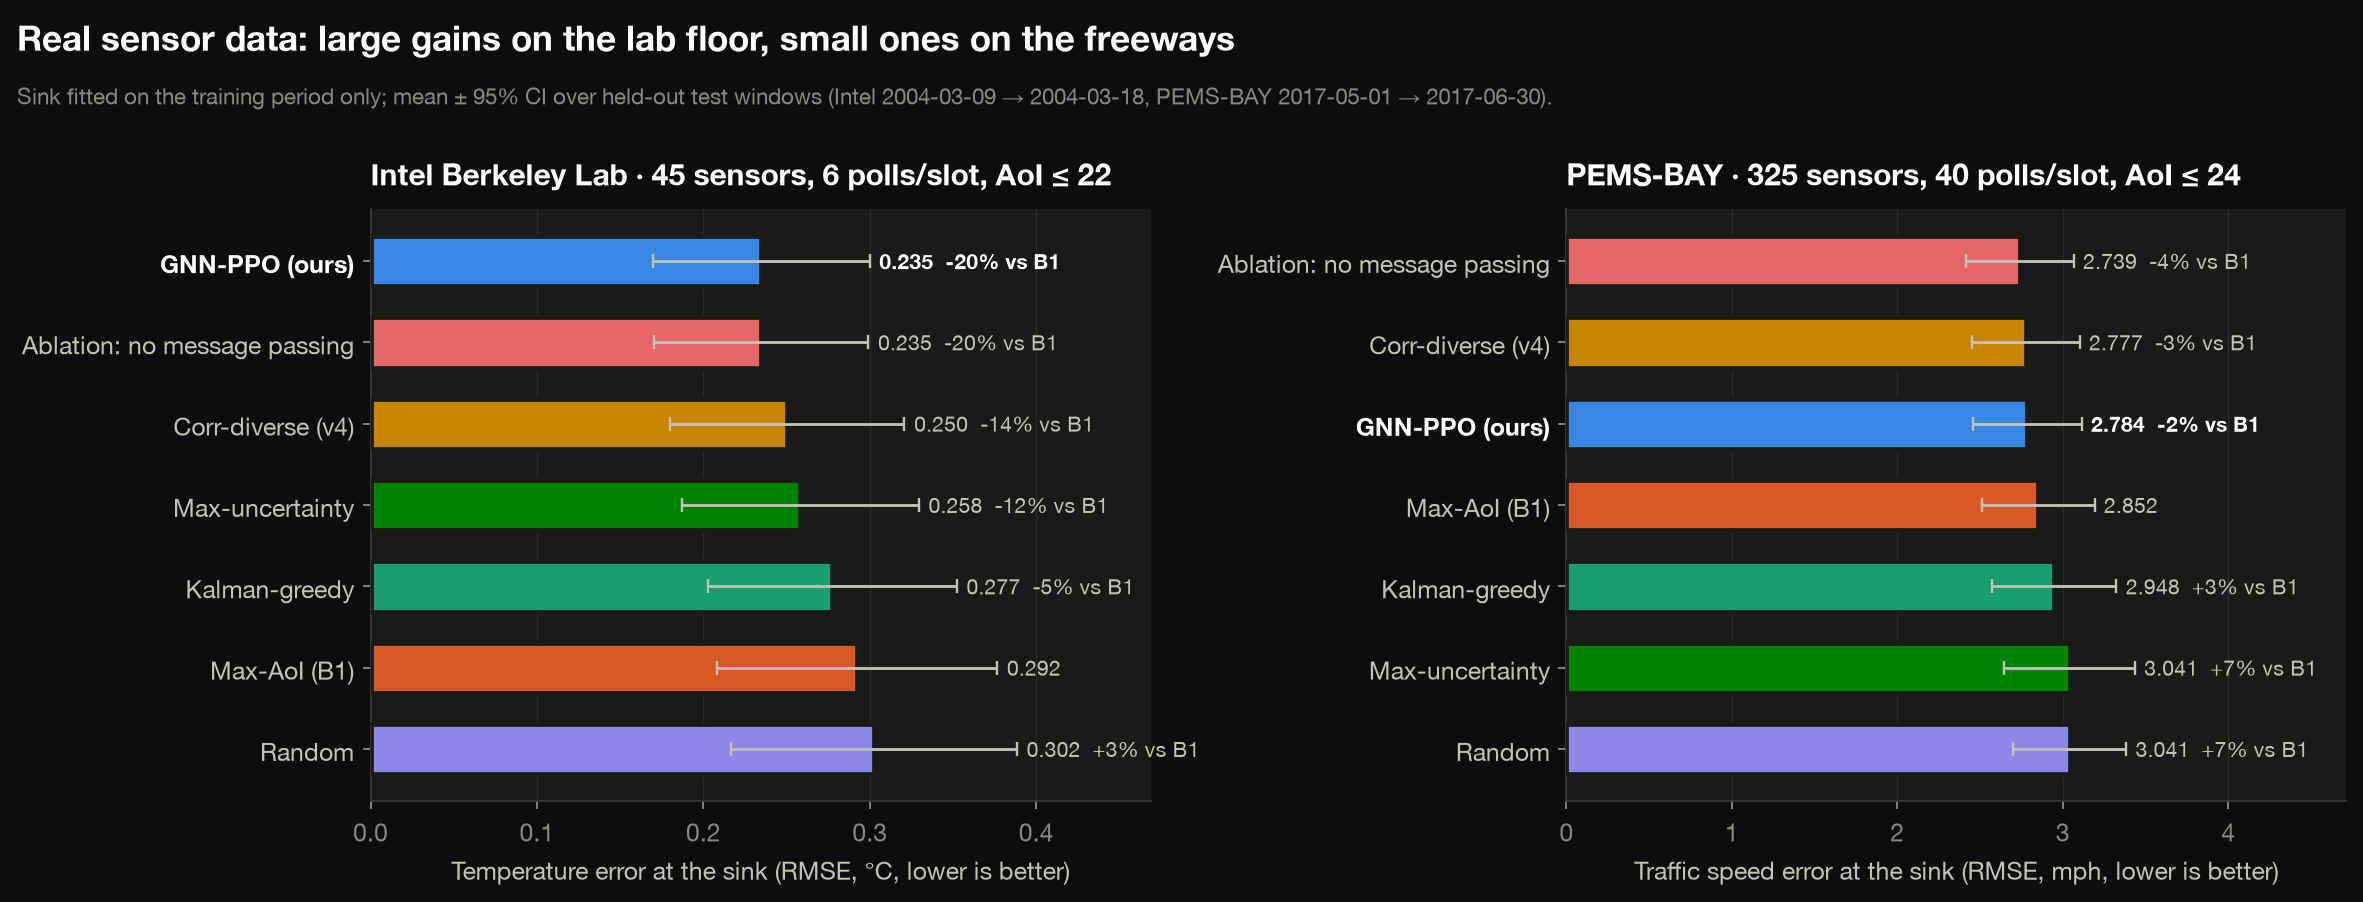
\includegraphics[width=\textwidth]{real_benchmark.png}
\caption{Sink RMSE on the held-out test periods. Left: Intel Lab (10 windows). Right: PEMS-BAY (15 windows).}\end{figure}

\begin{center}
\small
\begin{tabular}{@{}lcccc@{}}
\toprule
& \multicolumn{2}{c}{\textbf{Intel Lab} ($^\circ$C)} & \multicolumn{2}{c}{\textbf{PEMS-BAY} (mph)} \\
\textbf{Scheduler} & RMSE & mean AoI & RMSE & mean AoI \\
\midrule
Random & 0.302 & 6.72 & 3.041 & 7.27 \\
Max-AoI (B1) & 0.292 & 4.27 & 2.852 & 4.57 \\
Corr-diverse (v4) & 0.250 & 4.67 & 2.777 & 4.76 \\
Max-uncertainty & 0.258 & 5.37 & 3.041 & 6.28 \\
Kalman-greedy & 0.277 & 6.67 & 2.948 & 5.90 \\
\textbf{GNN-PPO (ours)} & \textbf{0.235} & 4.41 & \textbf{2.784} & 4.77 \\
Ablation (no message passing) & 0.235 & 4.40 & 2.739 & 4.69 \\
\bottomrule
\end{tabular}
\end{center}

\textbf{How to read it.} Each bar is a scheduler's average error over all test windows; the label shows the value and
the change against Max-AoI. Bars are sorted best at the top.

\textbf{Intel Lab.} The GNN has the lowest error, 0.235\,$^\circ$C, 20\% below Max-AoI and 15\% below Kalman-greedy. It wins
against Kalman-greedy in all 10 windows (Wilcoxon $p=0.002$) and against v4 in 8 of 10 ($p=0.05$). In standardised
MSE the GNN is 40.5\% below Max-AoI and 25.8\% below Kalman-greedy.

\textbf{PEMS-BAY.} Gains are smaller: the GNN is 2.4\% below Max-AoI in mph. Kalman-greedy is 3\% \emph{worse} than
Max-AoI: its fitted model is over-confident on traffic (it thinks it knows sensors it does not), so it neglects them.
The GNN, trained on real replays with the same kind of mismatch, does not fall into this; it beats Kalman-greedy in
15 of 15 windows ($p=6\times10^{-5}$). In standardised MSE the GNN is 10.7\% below Max-AoI and 13.4\% below
Kalman-greedy.

\begin{notebox}[Why the percentages in MSE and RMSE differ]
RMSE is the square root of MSE, which roughly halves a relative change (10\% lower MSE $\approx$ 5\% lower RMSE). And
RMSE in mph weights sensors by their natural variability: freeway sensors with large speed swings dominate, and those
are the hardest to infer from neighbours. Both numbers are correct; we report RMSE in units as the headline because it
is the error a user would see.
\end{notebox}

\begin{saybox}
``On the lab data, with the same 6 transmissions per 5 minutes and the same 2-hour freshness guarantee, our
scheduler's temperature error is 0.235 degrees against 0.292 for the classic scheduler, 20 percent lower, and it beats
the model-based greedy scheduler in every single test window. On the freeway data the improvement is smaller, 2.4
percent, because traffic sensors are less redundant, but it is still consistent: 15 out of 15 days.''
\end{saybox}

%-------------------------------------------------------------------------------
\subsection{Figure: real-data capacity and size sweeps}
\begin{figure}[H]\centering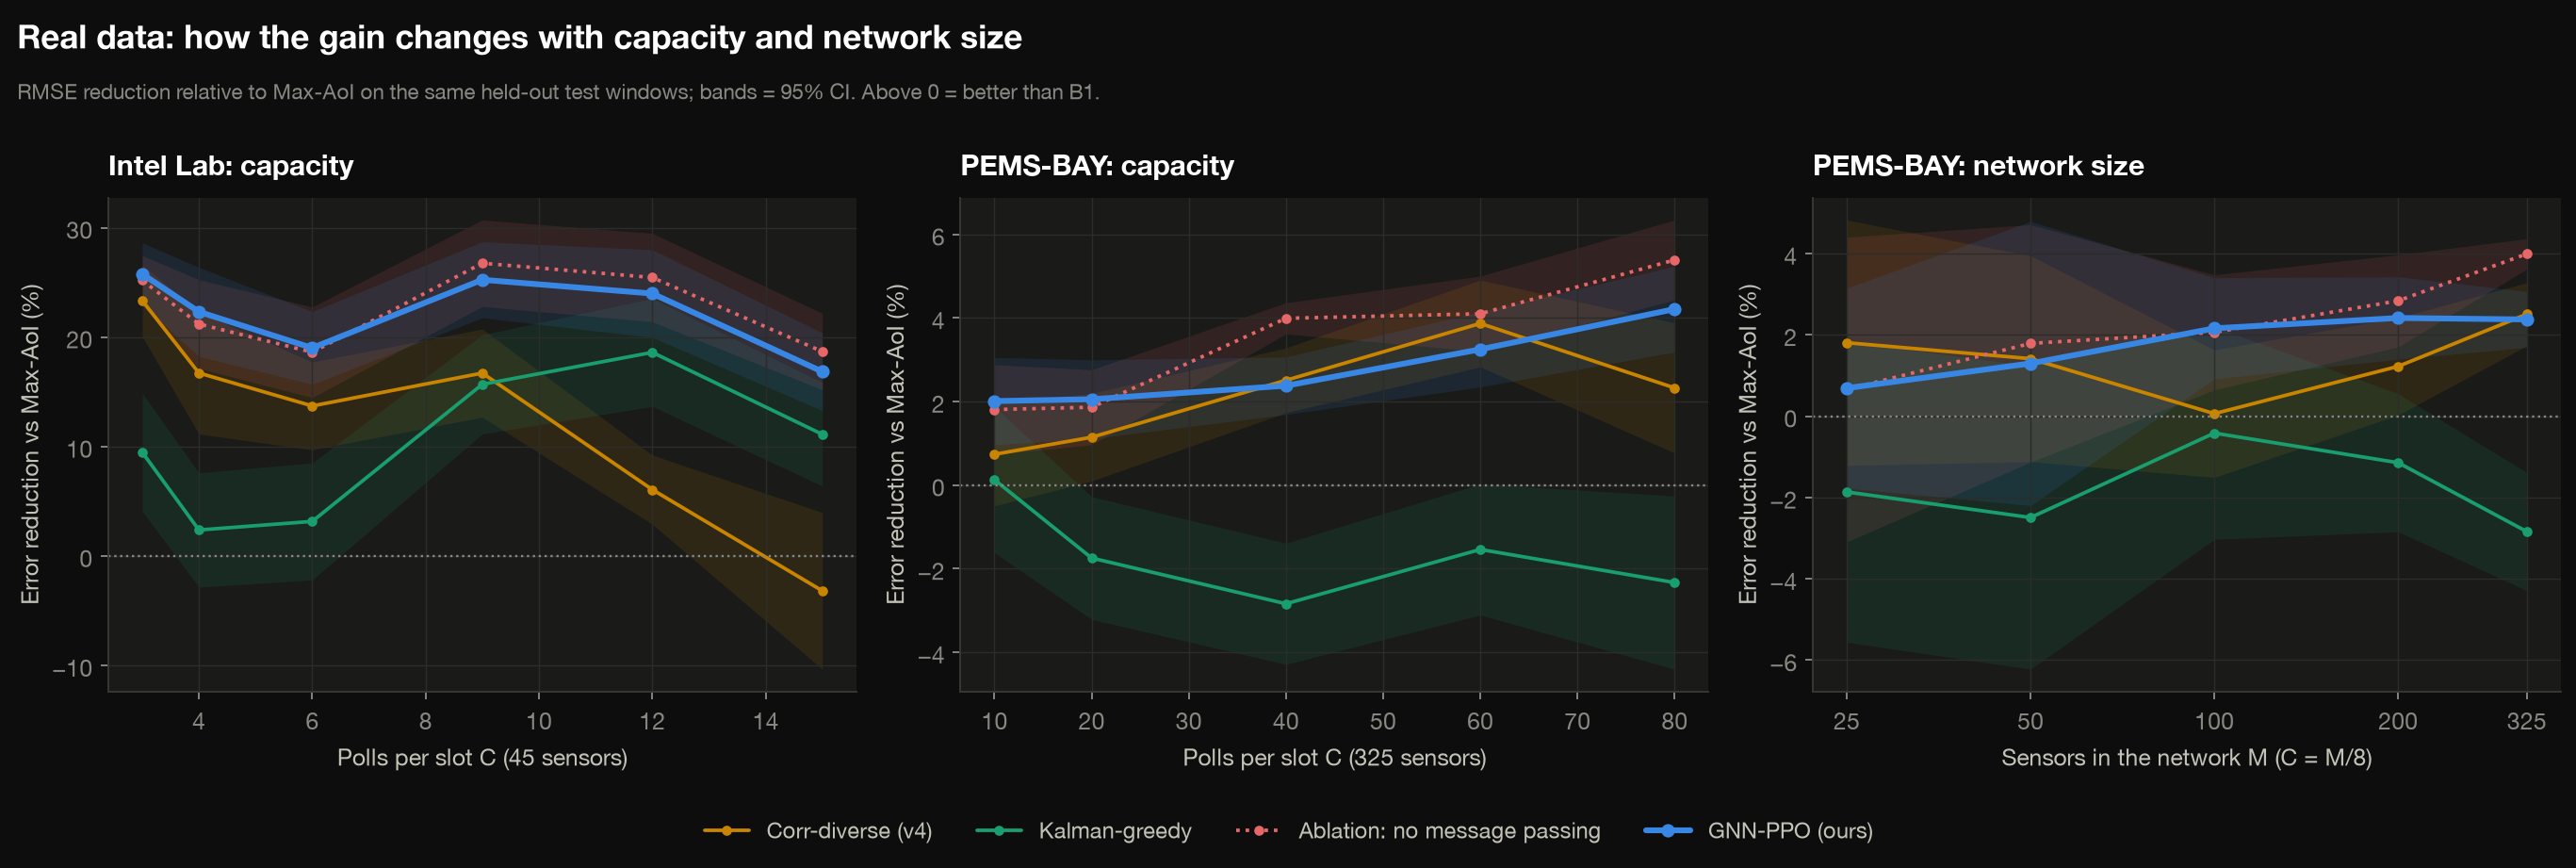
\includegraphics[width=\textwidth]{real_sweeps.png}
\caption{Error reduction against Max-AoI (above 0 = better) on real test windows, as capacity and network size vary.}\end{figure}

\textbf{How to read it.} The y-axis is ``percent less error than Max-AoI''. The dotted line at 0 means ``same as
Max-AoI''. Each line is a scheduler; the band is its 95\% CI.

\textbf{Left (Intel, capacity $C=3$ to 15).} The GNN (blue) stays 17--26\% better than Max-AoI at every capacity. The
heuristics are inconsistent: v4 drops below zero at $C=15$; Kalman-greedy ranges from 2\% to 19\%.

\textbf{Middle (PEMS-BAY, $C=10$ to 80).} The GNN's gain grows from 2\% to 4\% as capacity grows. Kalman-greedy is
below zero almost everywhere: model over-confidence again.

\textbf{Right (PEMS-BAY sub-networks of 25 to 325 sensors, $C=M/8$).} Gains are small (1--2.4\%) but positive and grow
with network size; larger networks have more neighbours to borrow information from.

\begin{saybox}
``The result is not tuned to one setting. On the lab data the gain stays between 17 and 26 percent for every channel
capacity we tried. On traffic it is small but grows with capacity and network size, while the model-based greedy
scheduler is actually worse than the classic one.''
\end{saybox}

%-------------------------------------------------------------------------------
\subsection{Figure: where each scheduler spends the channel}
\begin{figure}[H]\centering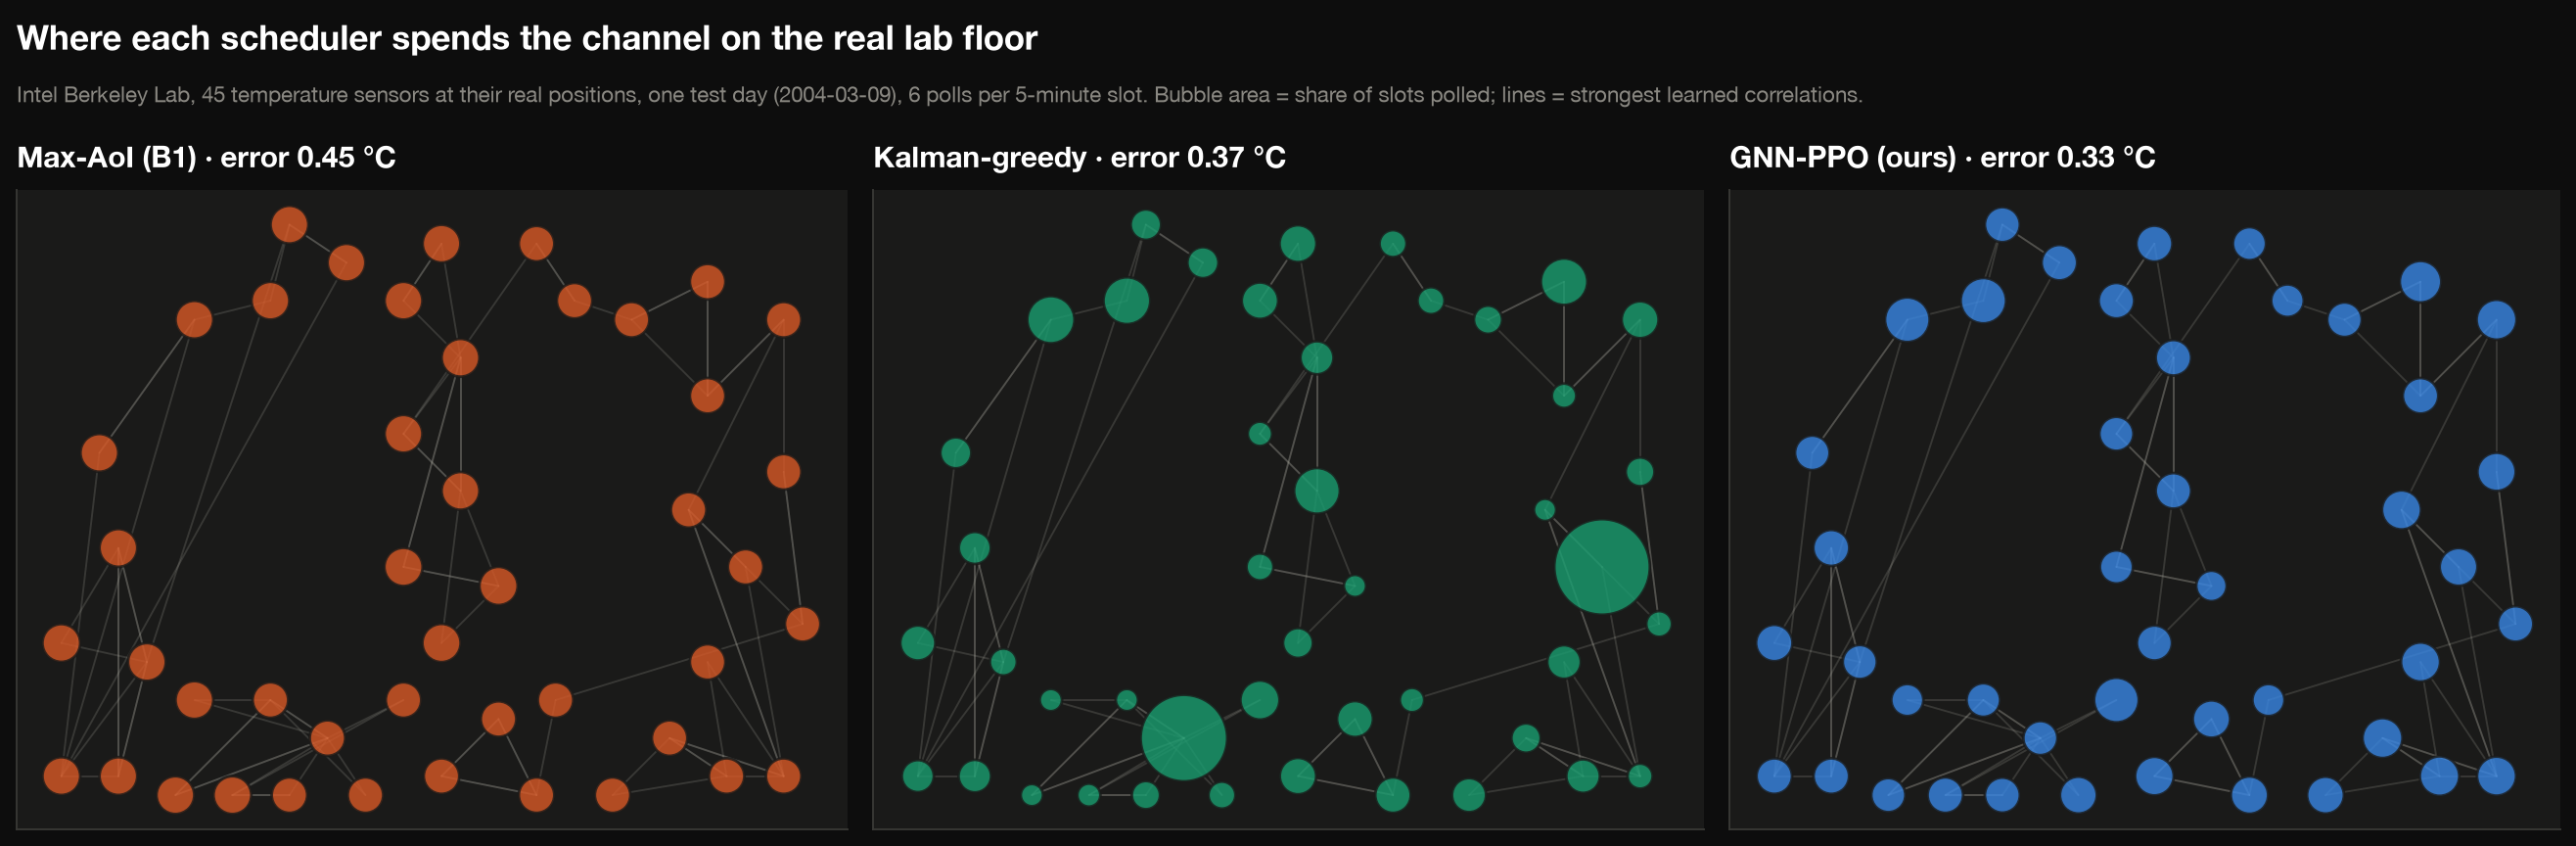
\includegraphics[width=\textwidth]{poll_map.png}
\caption{Intel Lab, one test day (9 March 2004). Bubble area = share of slots each sensor was polled.}\end{figure}

\textbf{What it shows.} Max-AoI (left) polls every sensor equally (round robin), error 0.45\,$^\circ$C. Kalman-greedy
(middle) concentrates on a few ``hub'' sensors (two huge bubbles) and polls many others only when the guard forces
it; error 0.37\,$^\circ$C. The GNN (right) spreads polls more evenly but not uniformly: more to sensors that are hard to infer,
fewer to sensors in dense, correlated groups; error 0.33\,$^\circ$C.

\begin{saybox}
``This shows \emph{how} each scheduler behaves. The classic one treats everyone equally. Greedy over-trusts its
model and fixates on a few sensors. Ours learned a balance: it polls each sensor according to how much the base
station can already guess about it.''
\end{saybox}

%-------------------------------------------------------------------------------
\subsection{Figure: synthetic benchmark}
\begin{figure}[H]\centering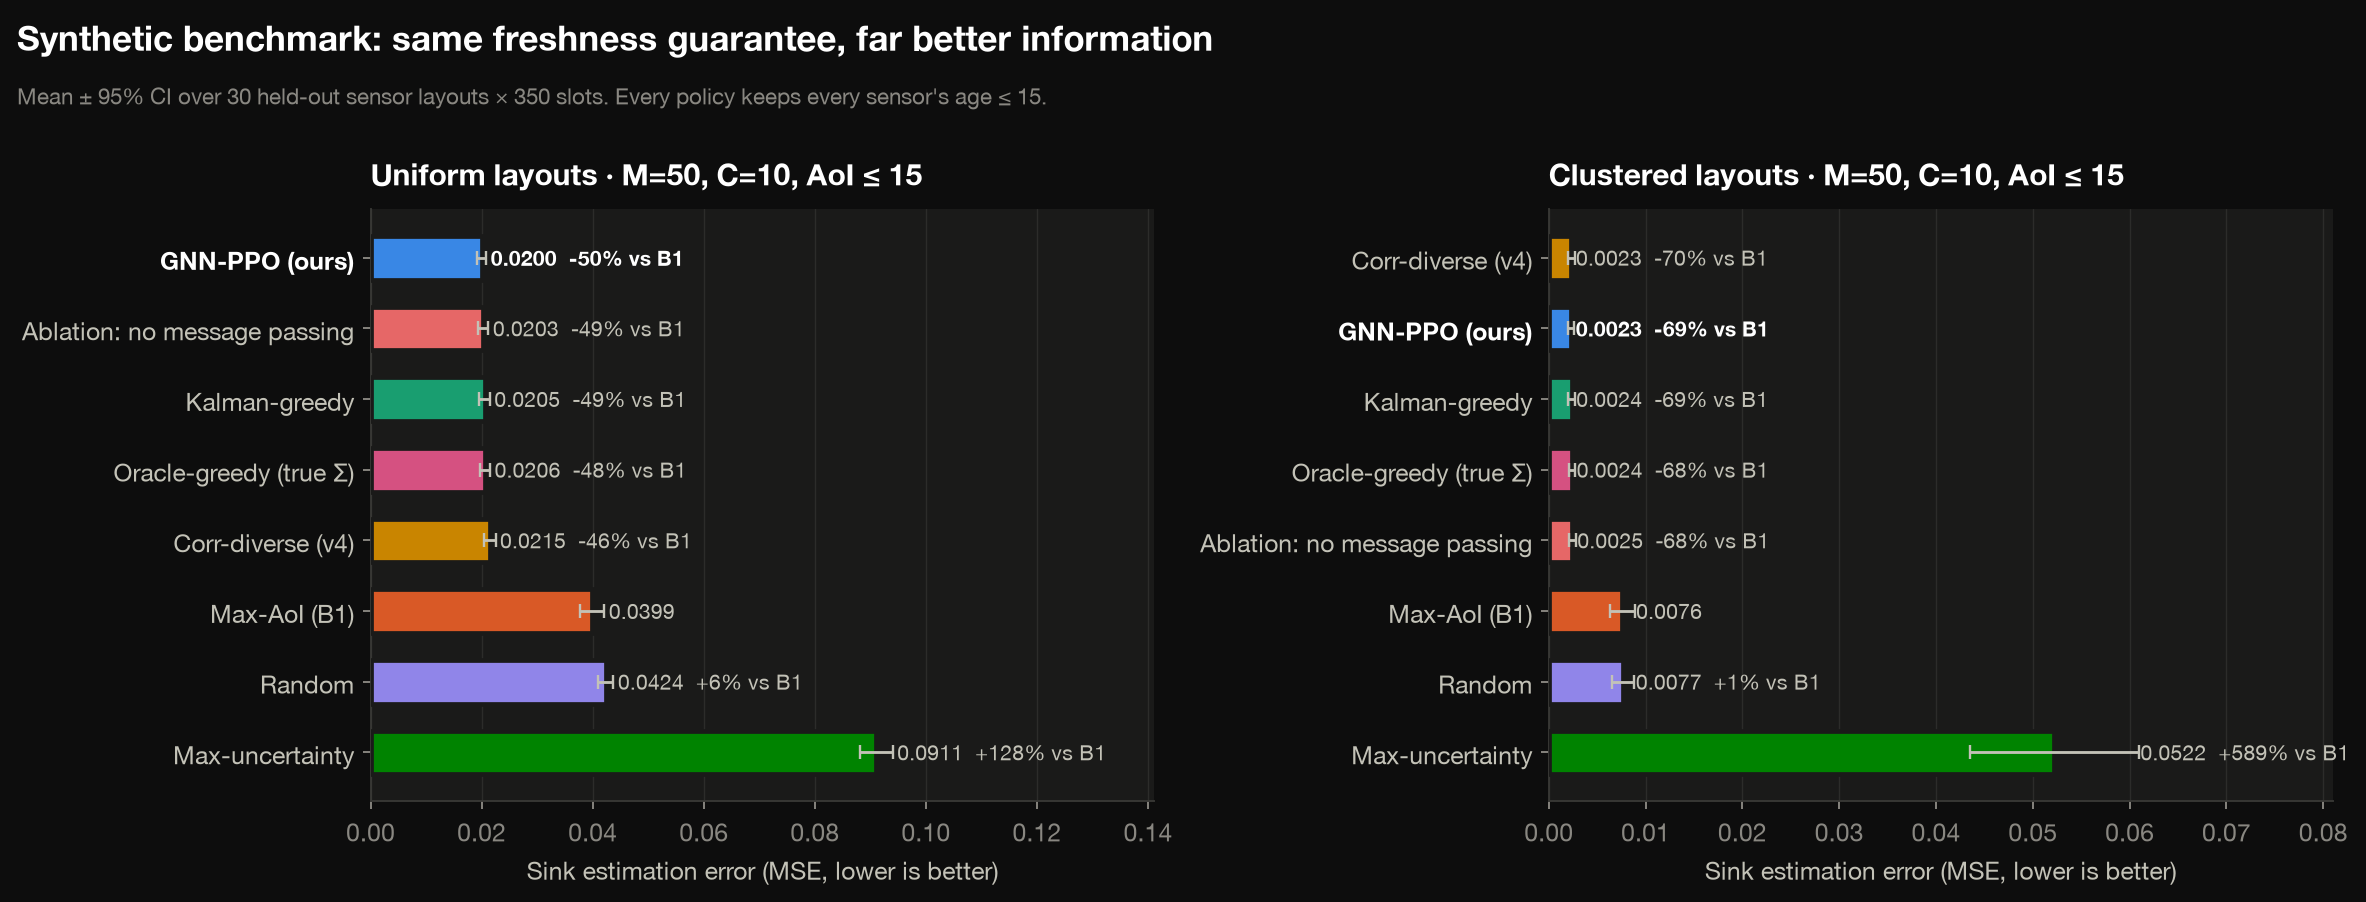
\includegraphics[width=\textwidth]{main_benchmark.png}
\caption{Synthetic fields, $M=50$, $C=10$, $F=15$, 30 unseen layouts $\times$ 350 scored slots.}\end{figure}

\textbf{Uniform layouts (left).} GNN MSE 0.0200, 50\% below Max-AoI (0.0399). It beats Kalman-greedy (0.0205) on 73\%
of layouts ($p=0.008$) and even the \emph{oracle} that knows the true covariance (0.0206) on 70\% ($p=0.003$). The
oracle is still greedy (one slot at a time); the GNN learned to look ahead. Max-uncertainty is the worst (0.0911):
polling the most uncertain sensors without considering overlap wastes polls on neighbours.

\textbf{Clustered layouts (right).} All correlation-aware schedulers reach about 0.0023--0.0024, 69\% below Max-AoI;
differences between them are not significant. In tight clusters any sensible correlation-aware rule finds the
redundancy.

\textbf{Ablation.} Removing message passing costs a little on synthetic data (GNN wins 67\% of uniform layouts and 87\%
of clustered layouts against the ablation).

\begin{saybox}
``In simulation we know the ground truth, so we can test many layouts. With the same freshness guarantee, our
scheduler halves the error of the classic scheduler, and it even beats a greedy scheduler that is given the true
correlations, because it learned to plan ahead instead of optimising one slot at a time.''
\end{saybox}

%-------------------------------------------------------------------------------
\subsection{Figure: fresher is not the same as better-informed}
\begin{figure}[H]\centering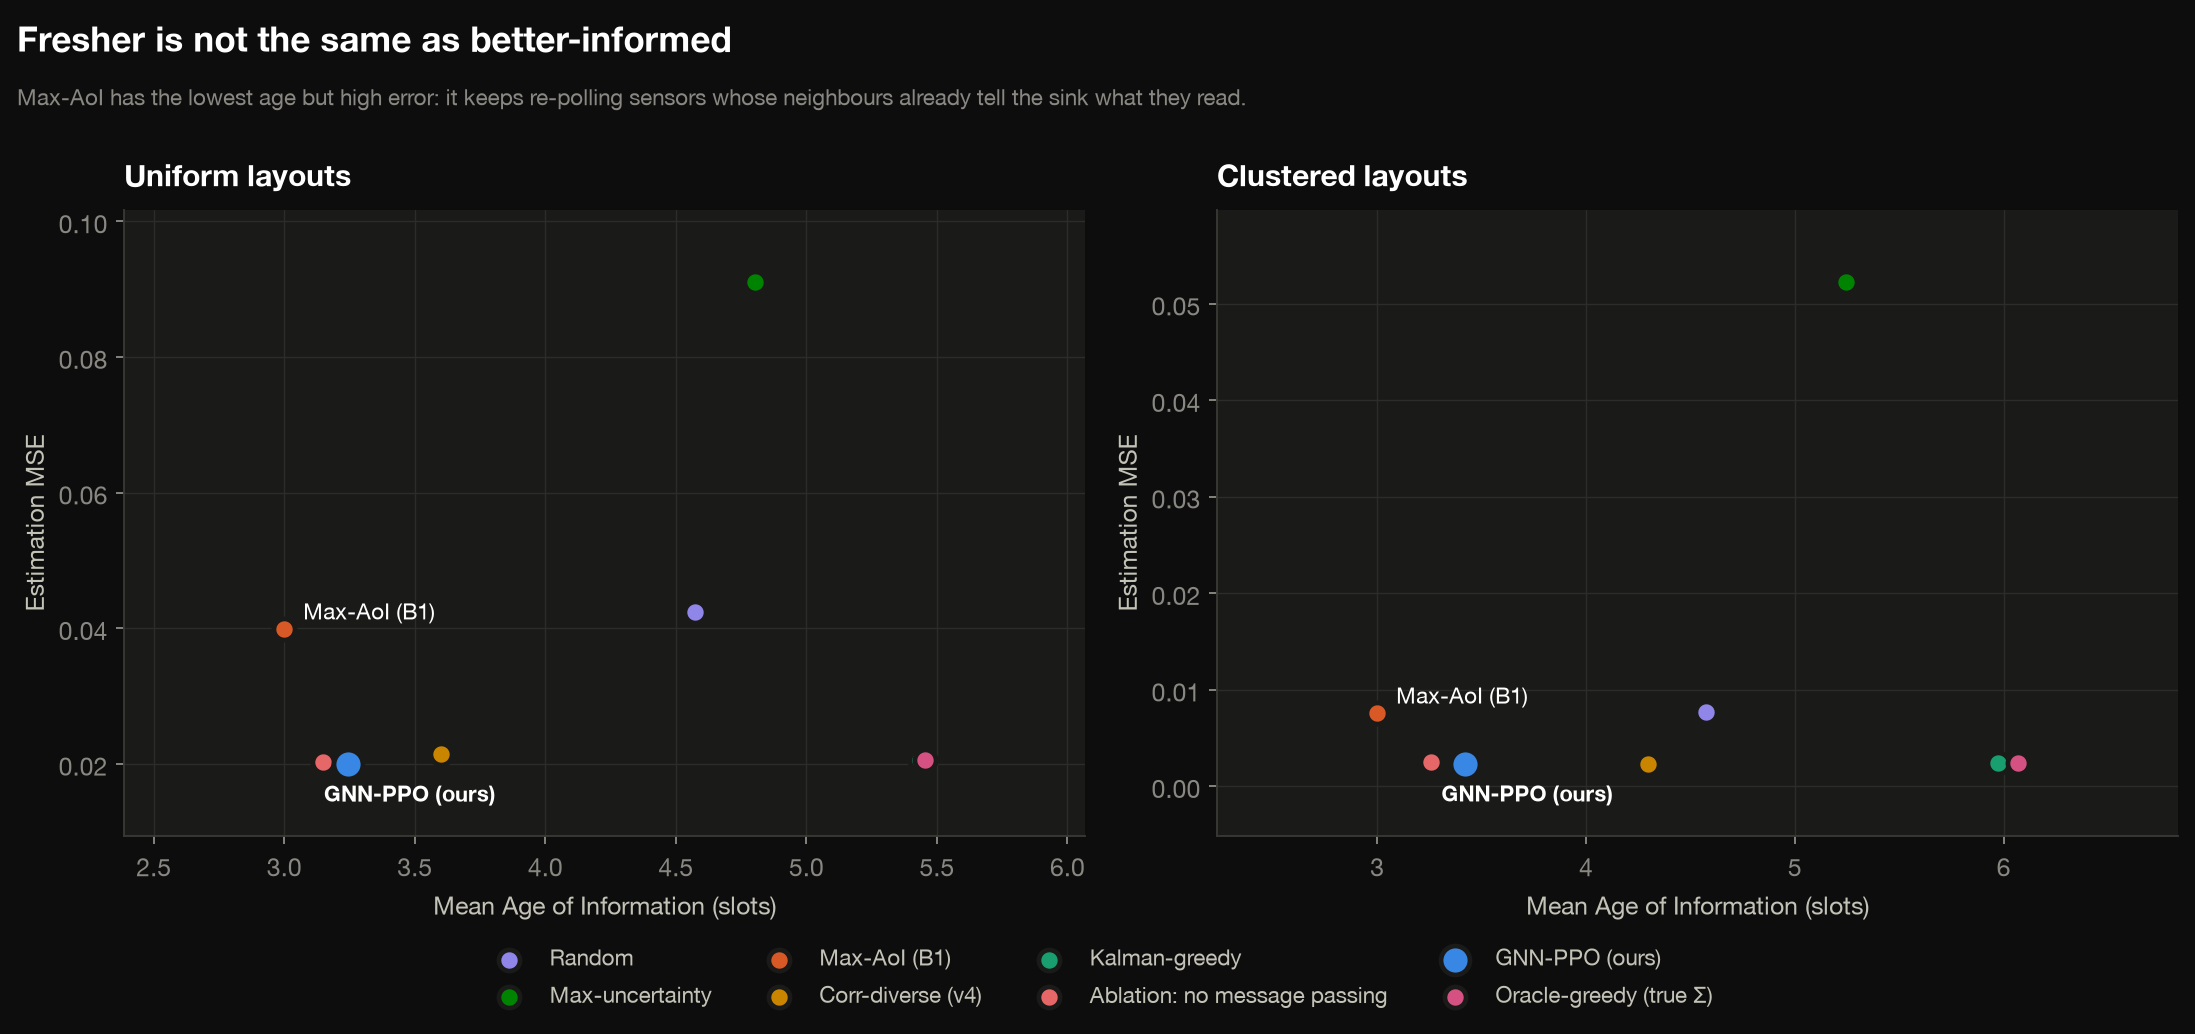
\includegraphics[width=\textwidth]{aoi_vs_error.png}
\caption{Each dot is a scheduler: mean AoI (x) against estimation error (y). Bottom-left is ideal.}\end{figure}

\textbf{What it shows.} Max-AoI has the \emph{lowest} age (3.0 slots) but about twice the error of the GNN. Kalman-greedy
and the oracle have low error but high age (5.4--6 slots): they let redundant sensors grow old. The GNN sits in the
bottom-left: low error \emph{and} low age (3.2--3.4).

\begin{saybox}
``This is the key insight of the project in one picture: minimising age is not the same as minimising error. The
classic scheduler is the freshest but not the best informed. Ours is nearly as fresh and far better informed.''
\end{saybox}

%-------------------------------------------------------------------------------
\subsection{Figure: synthetic sweeps}
\begin{figure}[H]\centering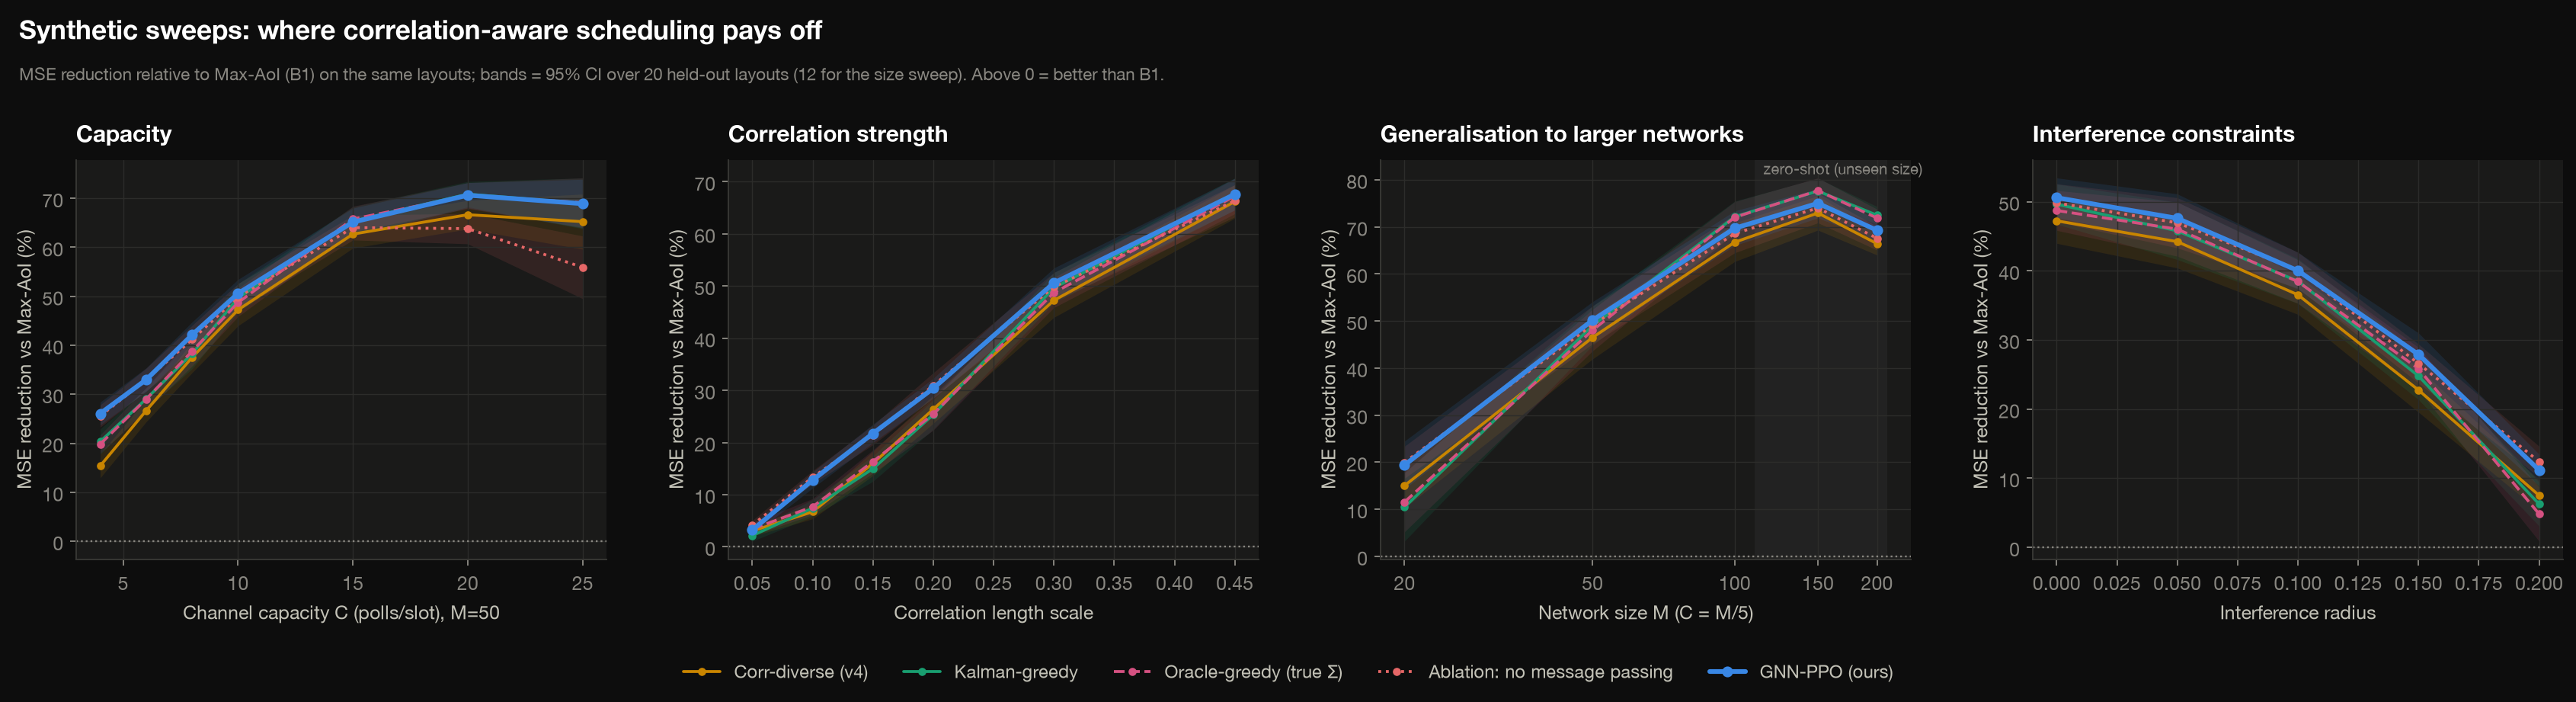
\includegraphics[width=\textwidth]{sweeps.png}
\caption{MSE reduction against Max-AoI as one setting changes at a time.}\end{figure}

\begin{itemize}
  \item \textbf{Capacity}: with very few polls ($C=4$), the GNN gains 26\% vs.\ 20\% for Kalman-greedy (GNN MSE 0.118 vs.\
        0.127): when the channel is scarce, planning matters most. The gain rises to about 70\% at $C=20$.
  \item \textbf{Correlation strength}: at length scale 0.05 (sensors almost independent) every method gains only about
        3\%: there is nothing to exploit. At 0.45 it is about 68\%. This confirms the gain really comes from
        correlation.
  \item \textbf{Network size}: training saw up to 100 sensors; 150 and 200 are \emph{zero-shot}. The GNN still gains about
        70\% vs.\ Max-AoI there, but Kalman-greedy and the oracle are 8--12\% better than the GNN for $M\ge100$.
  \item \textbf{Interference}: as more sensor pairs are forbidden to transmit together, every method's gain falls (51\%
        to 11\%) because the constraint itself forces spreading. The GNN stays at or near the top.
\end{itemize}

\begin{saybox}
``These sweeps check \emph{when} the idea works. If sensors are independent, nobody can do better than the classic
scheduler, and the curves show exactly that. The more correlated the sensors, and the scarcer the channel, the more
our approach helps.''
\end{saybox}

%-------------------------------------------------------------------------------
\subsection{Figure: how much history is needed}
\begin{figure}[H]\centering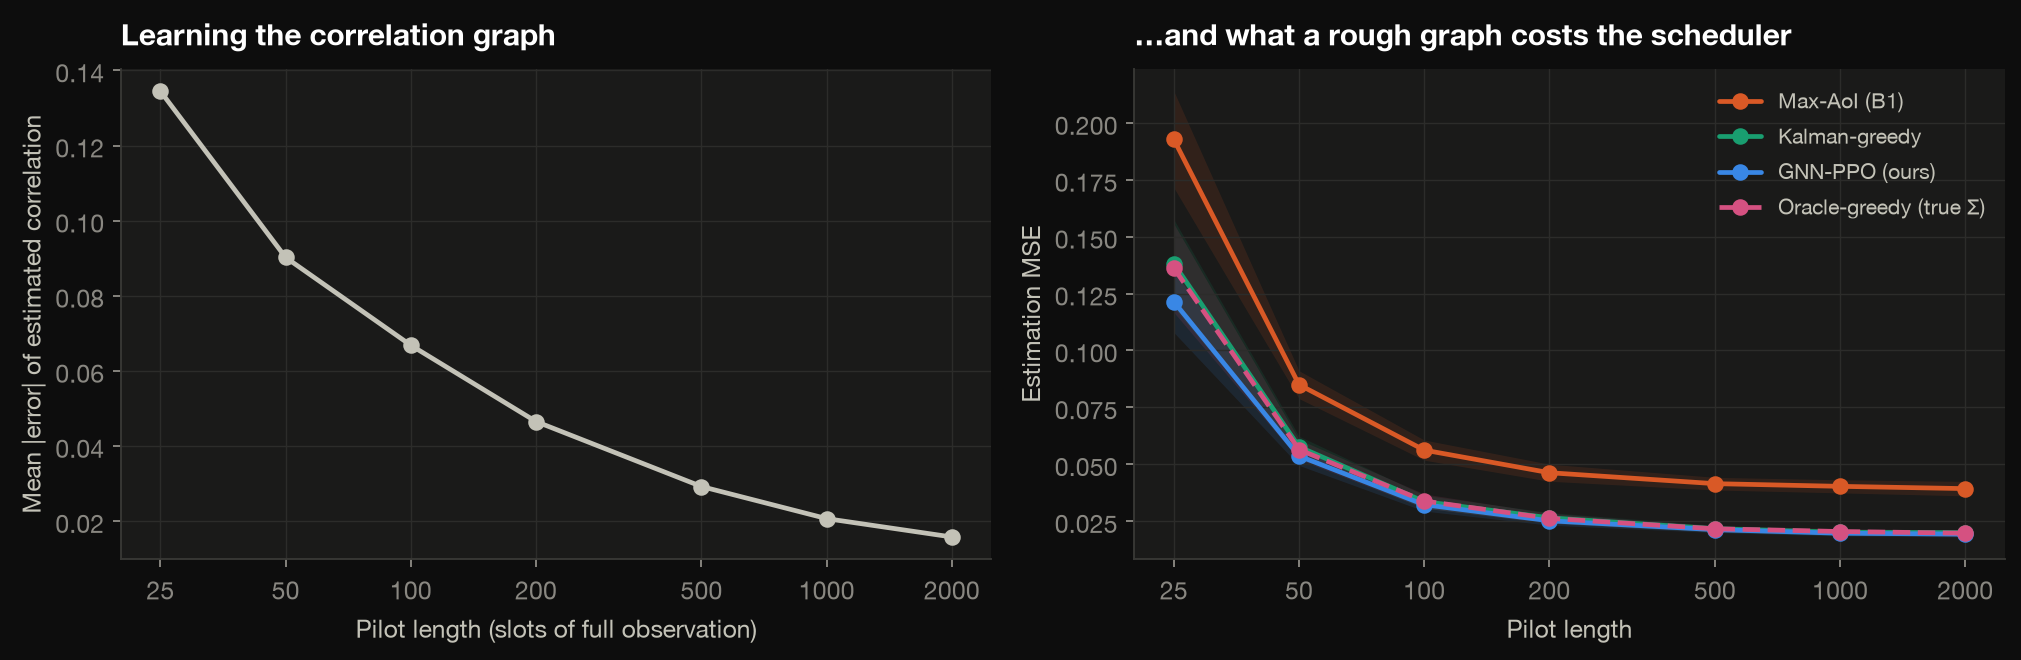
\includegraphics[width=\textwidth]{pilot_length.png}
\caption{Left: error of the learned correlations vs.\ length of the pilot (learning) phase. Right: the resulting
estimation error.}\end{figure}

\textbf{What it shows.} With only 25 slots of history the learned correlations are off by 0.135 on average; with 2000
slots, by 0.016. With rough correlations every scheduler suffers, but the GNN suffers least (MSE 0.122 vs.\ 0.138 for
Kalman-greedy at 25 slots) because it does not blindly trust the model. After about 500 slots (under two days of
5-minute data) results are close to their best.

\begin{saybox}
``How much data do we need before deploying? About 500 slots, less than two days of 5-minute readings. Even with less,
our scheduler degrades more gracefully than the model-based one.''
\end{saybox}

%-------------------------------------------------------------------------------
\subsection{Table: switching the freshness guard off}
\begin{center}
\small
\begin{tabular}{@{}lccc@{}}
\toprule
\textbf{Scheduler} ($M=50$, $C=10$, no guard) & \textbf{MSE} & \textbf{Sensors never polled} & \textbf{Max AoI} \\
\midrule
Max-AoI & 0.0399 & 0 & 5 \\
Corr-diverse (v4) & 0.0215 & 0 & 10.8 \\
Max-uncertainty & 0.1046 & 3.3 & 367.5 \\
Kalman-greedy & 0.0229 & \textbf{18} & \textbf{401} \\
Oracle-greedy & 0.0226 & \textbf{19.6} & \textbf{401} \\
\textbf{GNN-PPO (ours)} & \textbf{0.0200} & \textbf{0} & 10.3 \\
\bottomrule
\end{tabular}
\end{center}
A max AoI of 401 means a sensor was never polled in the whole 400-slot episode. Greedy schedulers abandon sensors they
can infer from neighbours. That is fine for the error number but unacceptable in practice: a sensor that breaks or
drifts would never be noticed. The GNN keeps the lowest error and still polls every sensor at least every 10--11 slots,
even without the guard.

\begin{saybox}
``Without our freshness rule, the greedy scheduler simply stops talking to 18 of the 50 sensors. If one of them failed,
nobody would know. Our scheduler gets lower error and still visits everyone, and with the guard on, freshness is
guaranteed for every scheduler.''
\end{saybox}

%-------------------------------------------------------------------------------
\subsection{Figure: training curves}
\begin{figure}[H]\centering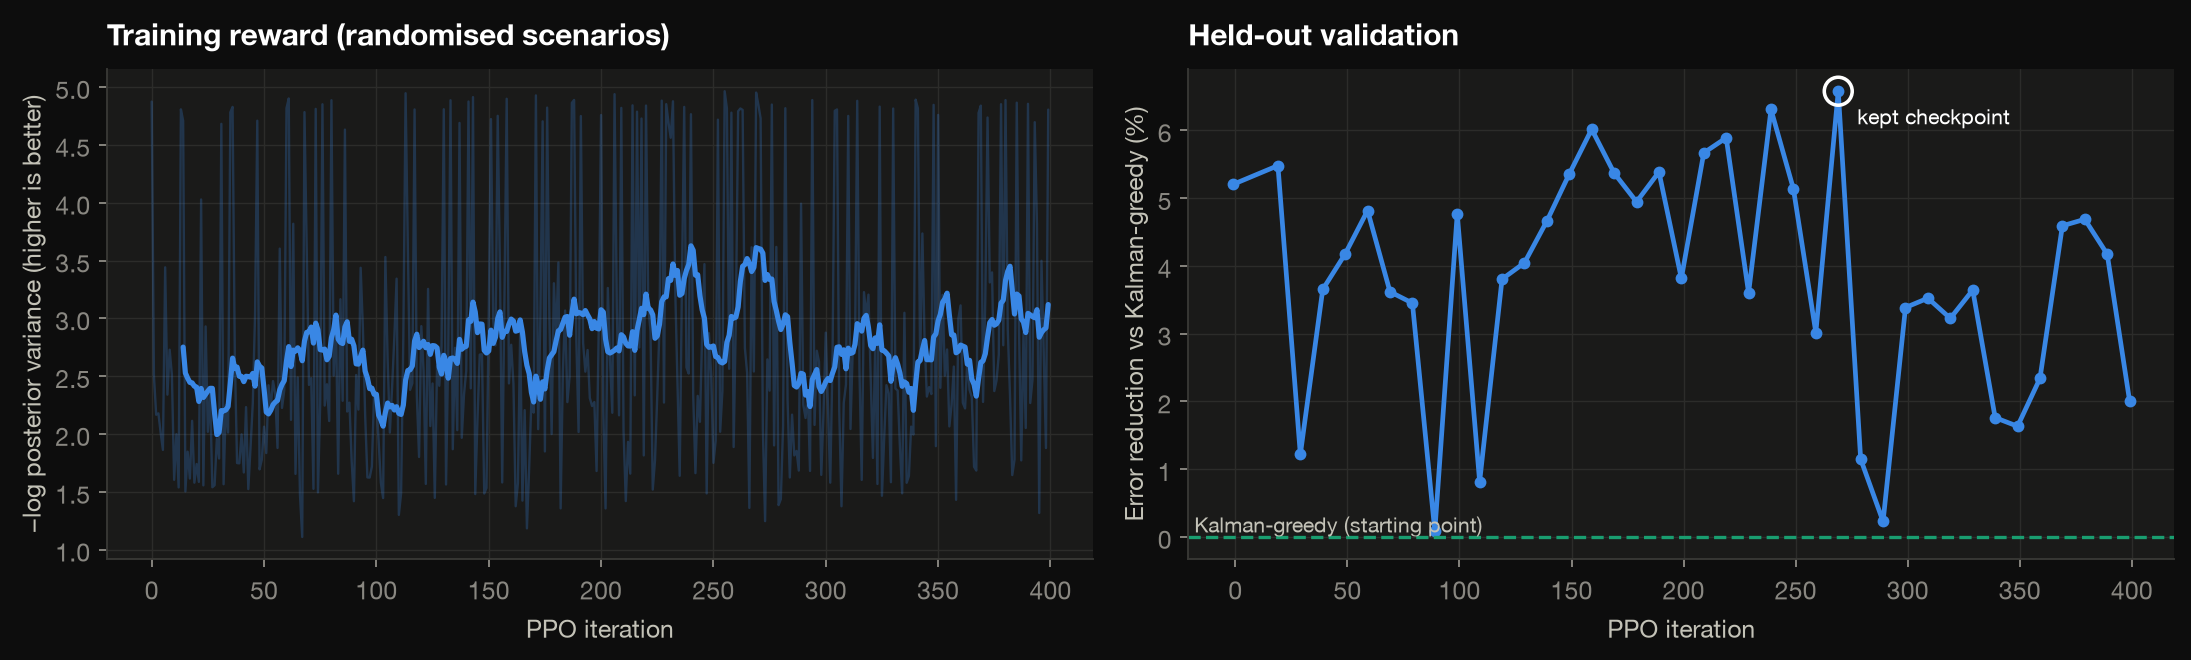
\includegraphics[width=\textwidth]{training.png}
\caption{Left: training reward. Right: validation improvement over Kalman-greedy.}\end{figure}

\textbf{Left.} Reward per PPO iteration (higher is better). It is noisy by design: each iteration uses a different
random network (size, capacity, correlation), so rewards differ a lot between iterations; the thick line is the
moving average, which trends upward.

\textbf{Right.} Held-out validation: how much lower the GNN's error is than Kalman-greedy's. The dashed line at 0 is
where training starts (the network \emph{is} Kalman-greedy at initialisation). It stays above 0 throughout and peaks at
+6.6\%; that checkpoint was kept.

\begin{saybox}
``Training starts exactly at the strongest classical scheduler, the dashed line, and every validation point after that
is better than it. We keep the best checkpoint, which is 6.6 percent better on held-out validation.''
\end{saybox}

%-------------------------------------------------------------------------------
\subsection{Figure: decision time}
\begin{figure}[H]\centering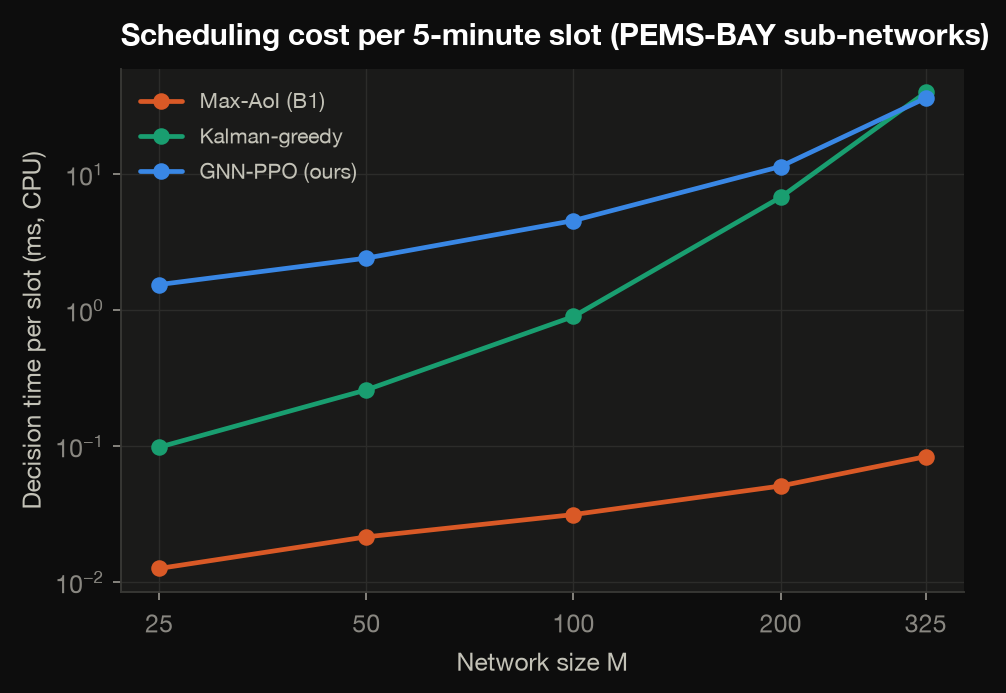
\includegraphics[width=0.6\textwidth]{decision_time.png}
\caption{Time to make one scheduling decision on a CPU, PEMS-BAY sub-networks (log scale).}\end{figure}

Max-AoI is almost free (under 0.1\,ms). Kalman-greedy grows steeply with size (0.1\,ms at 25 sensors to about 42\,ms at
325) because every pick updates the full covariance. The GNN costs 1.5\,ms at 25 sensors and about 37\,ms at 325, similar
to Kalman-greedy at full size. Either way, a decision takes less than a tenth of a second against a 300-second slot.

\begin{saybox}
``Even for 325 sensors a decision takes about 37 milliseconds on a laptop CPU, while a slot lasts 5 minutes, so the
scheduler easily runs in real time.''
\end{saybox}

%-------------------------------------------------------------------------------
\subsection{The live demo}
\begin{figure}[H]\centering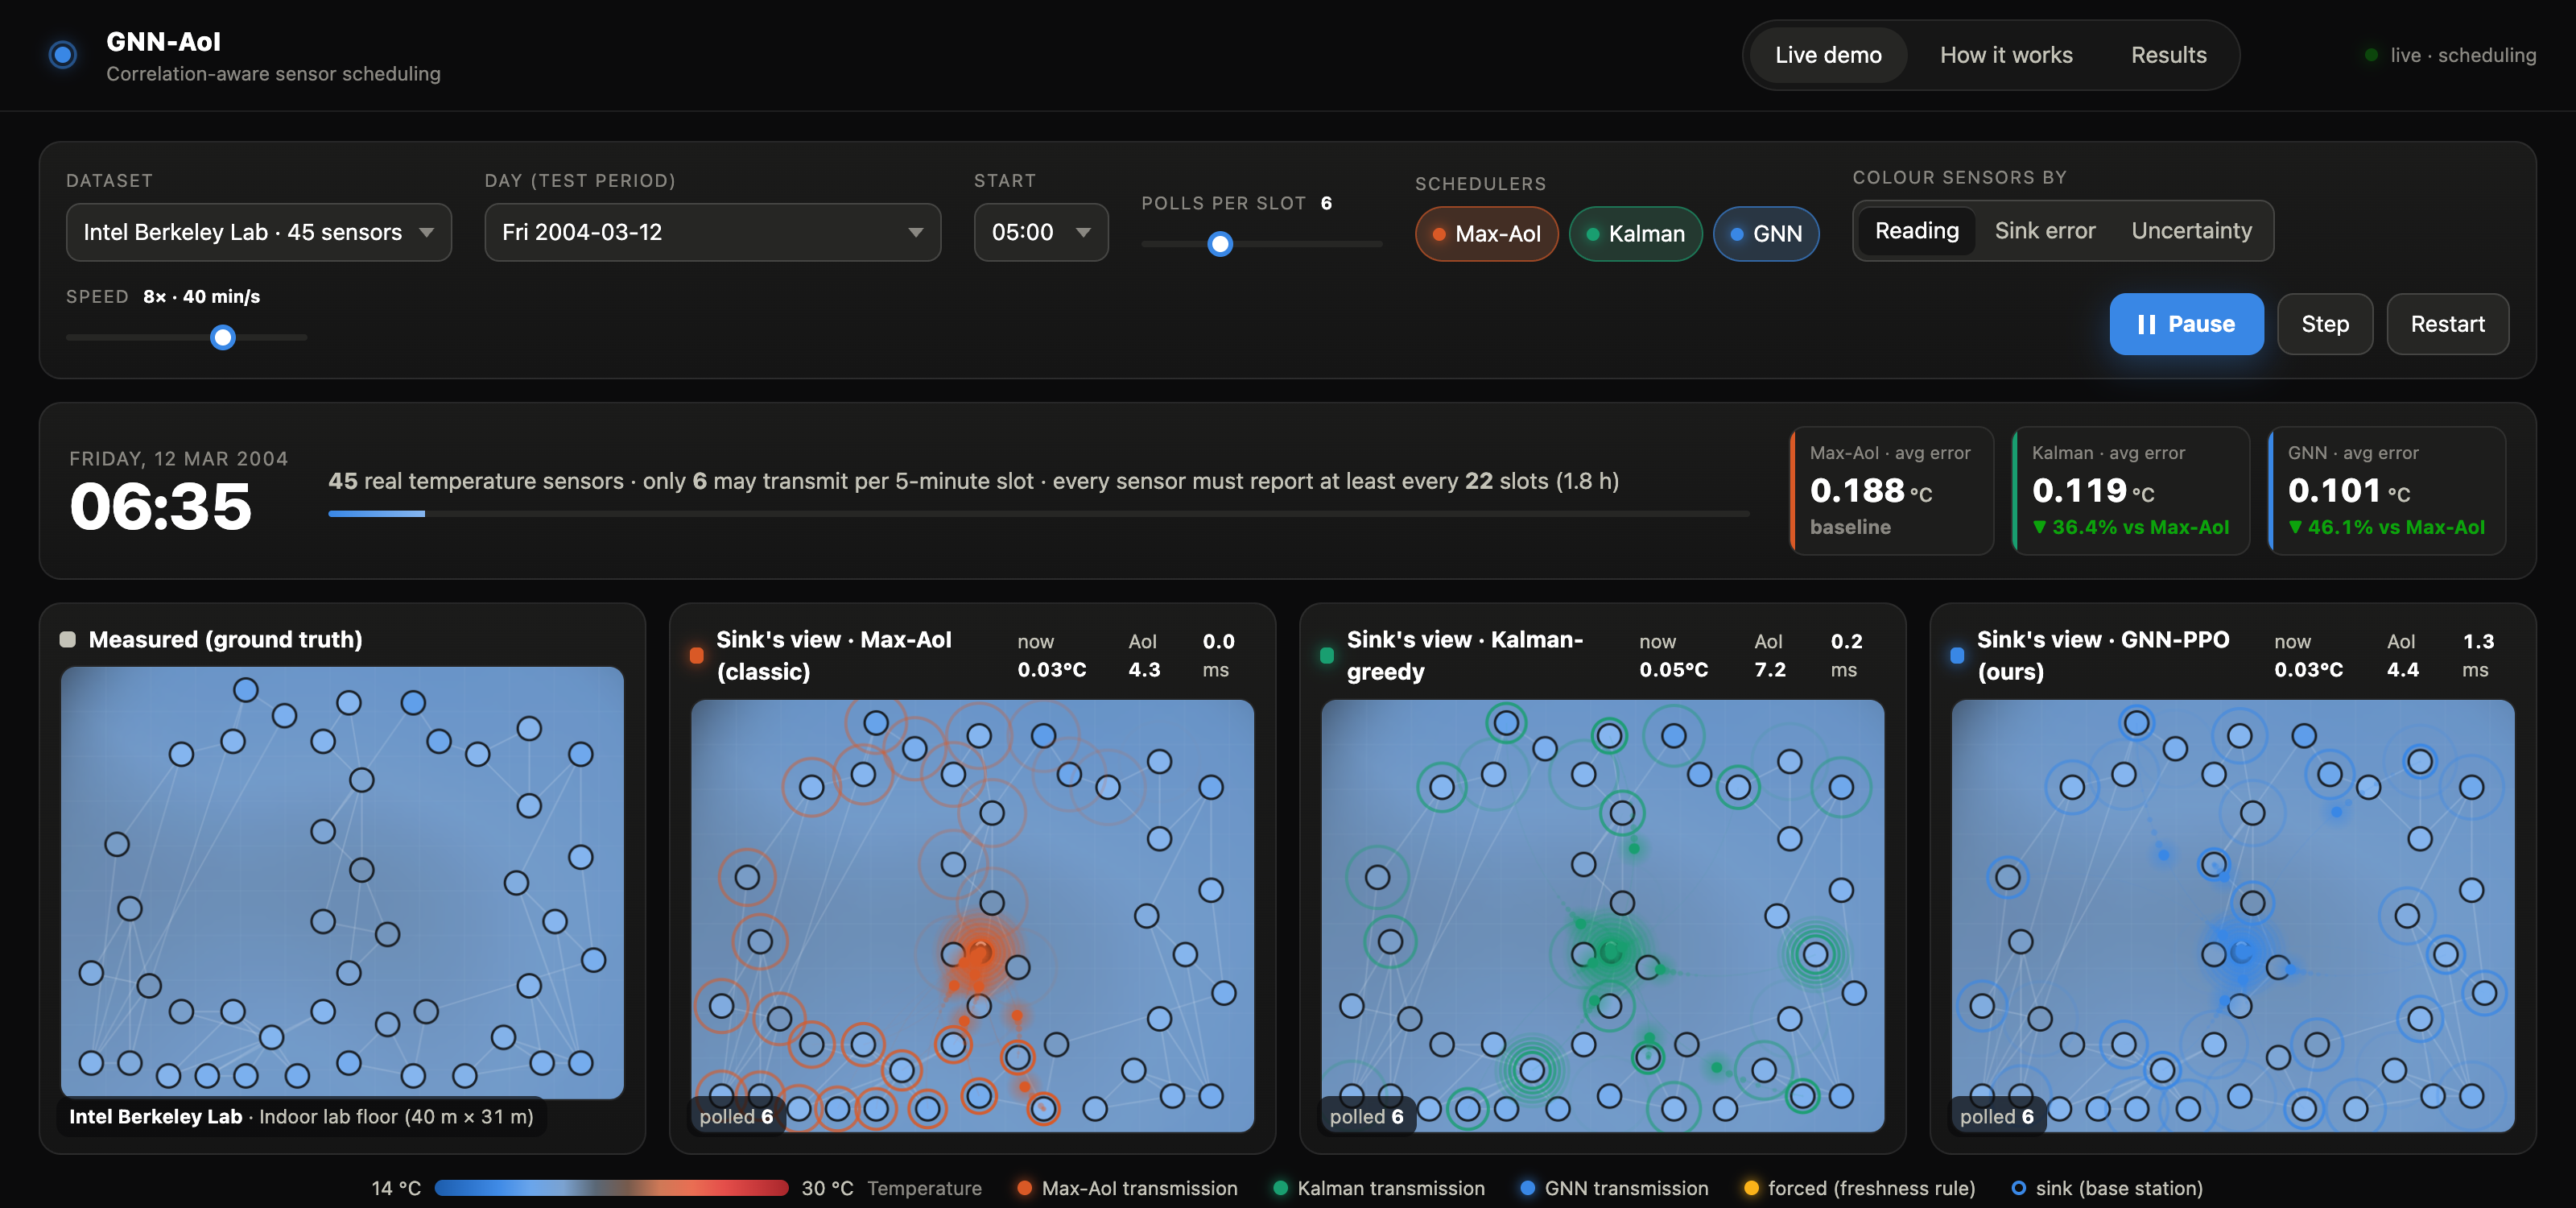
\includegraphics[width=\textwidth]{live_demo.png}
\caption{Live demo at \texttt{localhost:8000}, Intel Lab, Friday 12 March 2004, 06:35.}\end{figure}

\textbf{What each part shows.}
\begin{itemize}
  \item \textbf{Top controls}: dataset, test day, start hour, polls per slot, which schedulers to compare, how to colour
        sensors (reading, sink error, uncertainty), speed, play/step/restart.
  \item \textbf{Clock bar}: the real date and time being replayed and the running average error of each scheduler (here
        after 20 slots: Max-AoI 0.188\,$^\circ$C, Kalman 0.119\,$^\circ$C, GNN 0.101\,$^\circ$C, 46\% below Max-AoI).
  \item \textbf{Maps}: the measured floor, then each scheduler's view. Rings = sensors transmitting in this slot;
        a yellow ring = forced by the freshness rule.
  \item \textbf{Bottom}: error over time, ``Why these sensors?'' (the GNN's probability of picking each sensor first),
        and a transmission log listing which sensors each scheduler polled in each slot.
\end{itemize}

\begin{saybox}
``This is a real day from the test period, never used in training, replayed five minutes at a time. All three
schedulers see exactly the same readings. You can watch which six sensors each one polls, why the GNN chose them, and
how each base station's picture of the lab drifts from reality.''
\end{saybox}

\subsection{Comparison with recent literature}
\begin{center}
\small
\begin{tabularx}{\textwidth}{@{}p{3cm}XX@{}}
\toprule
\textbf{Work} & \textbf{Reported in their own setting} & \textbf{Same type of method on our real data} \\
\midrule
Ramakanth \emph{et al.}\ \cite{2} (base paper); Kadota \emph{et al.}\ \cite{16} & AoI-based scheduling within a constant factor of optimal & GNN lowers error 20\% (Intel) and 2.4\% (PEMS-BAY) vs.\ Max-AoI; wins 10/10 and 15/15 windows \\
Chen \emph{et al.}\ \cite{8} & Structure-enhanced DRL: 10--25\% lower MSE than benchmark DRL & GNN: 25.8\% (Intel) and 13.4\% (PEMS-BAY) lower MSE than Kalman-greedy \\
Krause \emph{et al.}\ \cite{19} & Greedy variance reduction is near-optimal per step & GNN beats it on 73\% of synthetic layouts, and beats it with the true covariance on 70\% \\
Reyhan \& Coleri \cite{9}; Farag \emph{et al.}\ \cite{7} & AoI limits met in probability & Hard bound, zero violations; greedy without a bound starves 18/50 sensors \\
\bottomrule
\end{tabularx}
\end{center}
The middle column comes from the cited papers' own setups and is not directly comparable; the right column re-runs that
class of method on our data under identical conditions.

\begin{saybox}[If the faculty asks: ``How do you compare with existing work?'']
``We cannot run their exact code on our data, so we re-implemented the type of method each paper uses: AoI-based
scheduling from our base paper and greedy uncertainty reduction from sensor-selection work. Under identical conditions,
on the same real test days, our scheduler beats both. Their own reported numbers are in a separate column so nobody
confuses the two.''
\end{saybox}

\section{Conclusion, limitations, future work and viva preparation}

\subsection{Limitations (state these honestly)}
\begin{itemize}
  \item \textbf{Ablation ties on real data.} On Intel Lab and PEMS-BAY, the model without message passing performs as
        well as the full GNN. The real-data gain comes mainly from the learned residual decoder (the correction on top of
        Kalman-greedy and the pairwise term); message passing helps measurably only on synthetic layouts.
  \item \textbf{Large networks.} On synthetic networks with 100 or more sensors (beyond the training range), Kalman-greedy
        is 8--12\% better than the GNN. Training on larger networks is the obvious fix.
  \item \textbf{Smaller gains on traffic.} PEMS-BAY sensors are less redundant than lab thermometers, so the gain is
        2.4\% in RMSE.
  \item \textbf{Model assumptions.} The sink assumes linear-Gaussian AR(1) dynamics; the channel is ideal apart from
        capacity and interference (no packet loss).
  \item \textbf{Offline training.} The correlation model is fitted once; it does not adapt if the environment changes.
\end{itemize}

\begin{saybox}[If asked: ``What does not work?'']
``Two things. On real data, removing the message passing does not hurt, so the improvement there comes from the
learned decoder rather than the graph layers. And on simulated networks larger than we trained on, plain Kalman-greedy is
still about 10 percent better. Both point to clear next steps.''
\end{saybox}

\subsection{Conclusion}
\begin{itemize}
  \item We identified, from the literature, that correlation-aware AoI work is analytical and hand-modelled, learned
        schedulers use interference graphs and soft freshness limits, and real-data evidence is scarce.
  \item We built \textbf{GNN-AoI}: a scheduler that learns the correlation structure from data, tracks the field with a
        Kalman sink, chooses transmissions with a GNN pointer decoder initialised as Kalman-greedy and trained with PPO,
        and guarantees every sensor's freshness by construction.
  \item On \textbf{real held-out data} it lowers the sink's error by \textbf{20\%} (Intel Lab, 45 sensors) and
        \textbf{2.4\%} (PEMS-BAY, 325 sensors) compared with AoI-based scheduling, and beats Kalman-greedy in
        \textbf{every} test window of both datasets.
  \item On simulated fields it halves the error of AoI scheduling and beats greedy selection that knows the true
        covariance.
  \item It runs in milliseconds, comes as a tested open-source package with reproducible experiments, and includes a
        live demo of real transmissions.
  \item The central lesson: \textbf{fresher is not the same as better-informed}. Using correlations to decide who
        transmits gives the sink a much better picture with the same channel, as long as freshness is still
        guaranteed.
\end{itemize}

\subsection{Future work}
\begin{itemize}
  \item Lossy channels with retransmissions (HARQ) \cite{6}.
  \item Online re-fitting of the correlation graph as seasons change or sensors are added.
  \item Training on larger networks; sparse message passing for thousands of sensors.
  \item Non-linear sinks (graph-recurrent forecasters such as DCRNN \cite{24}) in place of the Kalman filter.
  \item Distributed scheduling: each gateway runs the same shared GNN locally.
  \item A hardware pilot on a LoRa or Zigbee testbed.
\end{itemize}

\subsection{Likely viva questions}
\begin{description}[style=nextline,leftmargin=0.6cm]
  \item[What is Age of Information?] Slots since the sink last heard from a sensor. It measures freshness, not how much
        the sink knows.
  \item[Why not just minimise AoI?] Because correlated sensors make some transmissions redundant. Max-AoI has the
        lowest age but twice the error of our method (Figure ``fresher is not better-informed'').
  \item[What exactly does the GNN output?] A probability for each sensor at each pick step; the top choice is taken,
        the Kalman covariance is updated, and the next sensor is chosen, until the slot is full.
  \item[What is the reward?] $-(1-\gamma)\log(\text{error}+0.005)$ per slot: lower error, higher reward.
  \item[Why PPO and not DQN?] Choosing 6 of 45 sensors has millions of combinations; DQN needs a value per action. PPO
        trains our step-by-step selection policy directly and stably.
  \item[Why does the GNN start as Kalman-greedy?] So it never starts worse than the strongest classical method; RL only
        learns improvements. Behaviour cloning, which we tried first, never matched the teacher.
  \item[How do you guarantee freshness?] Sensors at age $F$ are forced into the slot before the scheduler acts; the
        environment asserts it every slot, and tests check every scheduler.
  \item[How do you avoid data leakage?] Chronological split; the profile, standardisation and model come only from the
        training period; validation uses separate data; a unit test checks it.
  \item[Why two datasets?] One with strong spatial correlation (indoor temperature), one large and less redundant
        (freeway traffic): they show where the method helps a lot and where it helps a little.
  \item[Why does Kalman-greedy lose on PEMS-BAY?] Its fitted model is over-confident: it believes it knows sensors it
        does not, so it polls them too rarely. Our policy saw this mismatch during training on real replays.
  \item[Is the improvement statistically significant?] Yes: Intel 10/10 windows vs.\ Kalman-greedy ($p=0.002$), PEMS-BAY
        15/15 ($p=6\times10^{-5}$), synthetic 73\% of layouts ($p=0.008$), Wilcoxon signed-rank tests.
  \item[How long does a decision take?] 4.6\,ms (Intel), 37\,ms (PEMS-BAY) on a laptop CPU; the slot is 5 minutes.
  \item[What is your base paper and what did you add?] Ramakanth, Tripathi \& Modiano, INFOCOM 2024. We add multiple polls
        per slot, correlations learned from data, a hard freshness bound, a learned GNN policy and real-data evaluation.
\end{description}

\subsection{References}\label{sec:refs}
{\small
\begin{enumerate}[label={[\arabic*]},leftmargin=1cm,itemsep=0.15em]
  \item V.~Tripathi and E.~Modiano, ``Optimizing age of information with correlated sources,'' \emph{Proc.\ ACM MobiHoc}, 2022, pp.~41--50; extended in \emph{IEEE/ACM Trans.\ Netw.}, vol.~32, no.~6, pp.~4660--4675, 2024.
  \item R.~V.~Ramakanth, V.~Tripathi, and E.~Modiano, ``Monitoring correlated sources: AoI-based scheduling is nearly optimal,'' \emph{Proc.\ IEEE INFOCOM}, 2024, pp.~641--650; extended in \emph{IEEE Trans.\ Mobile Comput.}, vol.~24, no.~2, pp.~1043--1054, 2025.
  \item E.~Erbayat, A.~Maatouk, P.~Zou, and S.~Subramaniam, ``Age of information optimization and state error analysis for correlated multi-process multi-sensor systems,'' \emph{Proc.\ ACM MobiHoc}, 2024, pp.~331--340.
  \item E.~Erbayat, A.~Maatouk, P.~Zou, and S.~Subramaniam, ``Age of information optimization with preemption strategies for correlated systems,'' \emph{Proc.\ IEEE ISIT}, 2025.
  \item M.~Fidler, F.~Gallistl, J.~P.~Champati, and J.~Widmer, ``2D-AoI: Age-of-information of distributed sensors for spatio-temporal processes,'' \emph{IEEE Trans.\ Commun.}, vol.~74, pp.~645--661, 2026.
  \item E.~T.~Ceran, D.~G\"und\"uz, and A.~Gy\"orgy, ``A reinforcement learning approach to age of information in multi-user networks with HARQ,'' \emph{IEEE J.\ Sel.\ Areas Commun.}, vol.~39, no.~5, pp.~1412--1426, 2021.
  \item H.~Farag, M.~Gidlund, and \v{C}.~Stefanovi\'c, ``A deep reinforcement learning approach for improving age of information in mission-critical IoT,'' \emph{Proc.\ IEEE GCAIoT}, 2021, pp.~14--18.
  \item J.~Chen, W.~Liu, D.~E.~Quevedo, Y.~Li, and B.~Vucetic, ``Structure-enhanced deep reinforcement learning for optimal transmission scheduling,'' \emph{Proc.\ IEEE ICC}, 2023, pp.~1212--1218.
  \item B.~G.~Reyhan and S.~Coleri, ``Safe deep reinforcement learning for resource allocation with peak age of information violation guarantees,'' \emph{IEEE Trans.\ Commun.}, vol.~73, no.~12, pp.~14197--14211, 2025.
  \item Y.~Shen, Y.~Shi, J.~Zhang, and K.~B.~Letaief, ``Graph neural networks for scalable radio resource management: Architecture design and theoretical analysis,'' \emph{IEEE J.\ Sel.\ Areas Commun.}, vol.~39, no.~1, pp.~101--115, 2021.
  \item Z.~Zhao, G.~Verma, C.~Rao, A.~Swami, and S.~Segarra, ``Link scheduling using graph neural networks,'' \emph{IEEE Trans.\ Wireless Commun.}, vol.~22, no.~6, pp.~3997--4012, 2023.
  \item L.~Wang, Q.~Wang, H.~Chen, and S.~Zhou, ``Age of information-oriented probabilistic link scheduling for device-to-device networks,'' \emph{Proc.\ IEEE/IFIP WiOpt}, 2024 (arXiv:2410.20196).
  \item W.~Wang, Q.~Wu, P.~Fan, N.~Cheng, W.~Chen, J.~Wang, and K.~B.~Letaief, ``Optimizing age of information in vehicular edge computing with federated graph neural network multi-agent reinforcement learning,'' \emph{IEEE Trans.\ Wireless Commun.}, vol.~25, pp.~23017--23032, 2026.
  \item R.~D.~Yates, Y.~Sun, D.~R.~Brown, S.~K.~Kaul, E.~Modiano, and S.~Ulukus, ``Age of information: An introduction and survey,'' \emph{IEEE J.\ Sel.\ Areas Commun.}, vol.~39, no.~5, pp.~1183--1210, 2021.
  \item S.~Kaul, R.~Yates, and M.~Gruteser, ``Real-time status: How often should one update?'' \emph{Proc.\ IEEE INFOCOM}, 2012, pp.~2731--2735.
  \item I.~Kadota, A.~Sinha, E.~Uysal-Biyikoglu, R.~Singh, and E.~Modiano, ``Scheduling policies for minimizing age of information in broadcast wireless networks,'' \emph{IEEE/ACM Trans.\ Netw.}, vol.~26, no.~6, pp.~2637--2650, 2018.
  \item A.~Maatouk, S.~Kriouile, M.~Assaad, and A.~Ephremides, ``The age of incorrect information: A new performance metric for status updates,'' \emph{IEEE/ACM Trans.\ Netw.}, vol.~28, no.~5, pp.~2215--2228, 2020.
  \item A.~S.~Leong, A.~Ramaswamy, D.~E.~Quevedo, H.~Karl, and L.~Shi, ``Deep reinforcement learning for wireless sensor scheduling in cyber--physical systems,'' \emph{Automatica}, vol.~113, art.~108759, 2020.
  \item A.~Krause, A.~Singh, and C.~Guestrin, ``Near-optimal sensor placements in Gaussian processes: Theory, efficient algorithms and empirical studies,'' \emph{J.\ Mach.\ Learn.\ Res.}, vol.~9, pp.~235--284, 2008.
  \item R.~E.~Kalman, ``A new approach to linear filtering and prediction problems,'' \emph{Trans.\ ASME J.\ Basic Eng.}, vol.~82, no.~1, pp.~35--45, 1960.
  \item T.~N.~Kipf and M.~Welling, ``Semi-supervised classification with graph convolutional networks,'' \emph{Proc.\ ICLR}, 2017.
  \item W.~Kool, H.~van Hoof, and M.~Welling, ``Attention, learn to solve routing problems!'' \emph{Proc.\ ICLR}, 2019.
  \item J.~Schulman, F.~Wolski, P.~Dhariwal, A.~Radford, and O.~Klimov, ``Proximal policy optimization algorithms,'' arXiv:1707.06347, 2017.
  \item Y.~Li, R.~Yu, C.~Shahabi, and Y.~Liu, ``Diffusion convolutional recurrent neural network: Data-driven traffic forecasting,'' \emph{Proc.\ ICLR}, 2018 (PEMS-BAY dataset).
  \item P.~Bodik, W.~Hong, C.~Guestrin, S.~Madden, M.~Paskin, and R.~Thibaux, ``Intel Lab Data,'' 2004. Online: \url{http://db.csail.mit.edu/labdata/labdata.html}
\end{enumerate}
}


\end{document}
